% How accurate LIGHT_ArF is: v0_2 (0-D) and 1Dv0_2 (1-D) against the ArF
% measurements, with their reaction rates (Appendix A) and the data scored
% (Appendix B). No model number here is typed by hand. They come from three
% generated files and the figures, all written by make_overview.py:
%   overview_rates.tex    the network (v0_2/network.py, species.py)
%   overview_scores.tex   arf_data/score_0d.json and score_1d.json
%   overview_runs.tex     fresh runs of v0_2 and 1Dv0_2
%   energy_ladder.tex     make_energy_ladder.py
%   system_map_numbers.tex, system_map.pdf   make_system_map.py, then
%                         latexmk -pdf system_map.tex
%   figures/*.pdf
% Build from Kinetic_Modeling/:
%   python3 LIGHT_ArF_ebeam/docs/make_overview.py
%   ~/.venvs/f2sweep/bin/python LIGHT_ArF_ebeam/docs/make_overview.py --runs
%   cd LIGHT_ArF_ebeam/docs && /opt/homebrew/bin/latexmk -pdf accuracy_overview.tex
\documentclass[11pt]{article}
\usepackage[a4paper,margin=2.2cm]{geometry}
\usepackage[T1]{fontenc}
\usepackage[scaled=0.95]{helvet}
\renewcommand{\familydefault}{\sfdefault}
\usepackage{amsmath}
\usepackage{sansmath}
\usepackage{booktabs,tabularx,array,longtable}
\usepackage{xcolor}
\usepackage{graphicx}
\usepackage{float}
\usepackage{enumitem}
\usepackage{needspace}
\usepackage[hyphens]{url}
\usepackage{tikz}
\usetikzlibrary{arrows.meta,decorations.pathmorphing}
\usepackage{pdfpages}
\setlist{nosep, leftmargin=1.2em}
\setlength{\parindent}{0pt}
\setlength{\parskip}{5pt}

% chemistry and units (the generated tables use these)
\newcommand{\unit}[1]{\ensuremath{\,\mathrm{#1}}}
\newcommand{\el}{\ensuremath{\mathrm{e}^-}}
\newcommand{\Ars}{Ar\ensuremath{^*}}
\newcommand{\Arp}{Ar\ensuremath{^+}}
\newcommand{\Artp}{Ar\ensuremath{_2^+}}
\newcommand{\Arts}{Ar\ensuremath{_2^*}}
\newcommand{\AtF}{Ar\ensuremath{_2}F\ensuremath{^*}}
\newcommand{\ArFs}{ArF\ensuremath{^*}}
\newcommand{\Ft}{F\ensuremath{_2}}
\newcommand{\Fm}{F\ensuremath{^-}}
\newcommand{\ra}{\ensuremath{\to}}
\newcommand{\hnu}{\ensuremath{h\nu}}
\newcommand{\gIP}{\ensuremath{g_0I_\mathrm{sat}/P}}
\newcommand{\Edep}{\ensuremath{E_\mathrm{dep}}}
\newcommand{\x}[1]{\ensuremath{\times}#1}
% a factor of the measurement as a percentage of it (0.64 -> 64), as LIGHT's
% overview prints it: \pctof{x} to the unit, \pctof[1]{x} to a tenth
\newcommand{\pctof}[2][0]{\pgfmathparse{100*#2}%
  \pgfmathprintnumber[fixed,precision=#1]{\pgfmathresult}}

% LIGHT_ArF_ebeam reaction-rate tables. GENERATED by make_overview.py from LIGHT_ArF_ebeam
% v0_2 0.2.0-arf-ebeam. Do not edit. Rerun the script instead.
\providecommand\widef[2]{\expandafter\def\csname wi@#1\endcsname{#2}}
\widef{version}{0.2.0-arf-ebeam}
\widef{rates.nBasic}{69}
\widef{rates.nGroup}{5}
\widef{rates.nBands}{14}
\widef{rates.nAr}{37}
\widef{rates.nAr4s}{4}
\widef{rates.nArHi}{33}
\widef{rates.nBandRows}{13}
\widef{rates.nZero}{5}
\widef{rates.tauB}{4.2}
\widef{rates.ebreak}{11.548}
\widef{rates.temax}{30}
\widef{beam.W}{25.2}
\widef{beam.exc}{0.39}
\widef{beam.eps}{4.4}
\widef{beam.W0}{25.2}
\widef{beam.ceil}{0.538}
\widef{beam.Wlit}{26.4}
\widef{beam.Wmiss}{4.5}
\widef{beam.rebW}{30.85}
\widef{beam.rebexc}{0.84}
\widef{beam.ebar}{10.0}
\def\wiTRows{%
G1\_3P2 to G1\_1P1 & \el{} + Ar \ra{} \el{} + \Ars{}, the four 4s levels, 11.548 to 11.828 eV & $\langle\sigma v\rangle$ & $T_e$, $T_\mathrm{tail}$ & IST-Lisbon set, Yanguas-Gil, Cotrino and Alves 2005\\
C1\_4p01 to C1\_4dp & \el{} + Ar \ra{} \el{} + Ar(4p, 3d, 5p, 5s, 4d, 6s) \ra{} \Ars{}, 33 levels, 12.907 to 14.967 eV & $\langle\sigma v\rangle$ & $T_e$, $T_\mathrm{tail}$ & IST-Lisbon set, prompt cascade to 4s after Setser 1977\\
C2 & \el{} + Ar \ra{} 2\el{} + \Arp{} & $\langle\sigma v\rangle$ & $T_e$, $T_\mathrm{tail}$ & IST-Lisbon set, Rapp and Englander-Golden\\
G6 & \el{} + Ar, elastic & energy loss & $T_e$, $T_g$ & IST-Lisbon momentum transfer, after Phelps\\
ATT & \el{} + \Ft{} \ra{} \Fm{} + F & $\langle\sigma v\rangle$ & $T_e$ & SIGLO\\
DIS\_a3 & \el{} + \Ft{} \ra{} \el{} + 2F & $\langle\sigma v\rangle$ & $T_e$ & SIGLO\\
DIS\_A1 & \el{} + \Ft{} \ra{} \el{} + 2F & $\langle\sigma v\rangle$ & $T_e$ & SIGLO\\
VIB1 to VIB4 & \el{} + \Ft{} \ra{} \el{} + \Ft{}($v$ = 1 to 4) & $\langle\sigma v\rangle$ & $T_e$ & SIGLO\\
G2 & 2\Ars{} \ra{} \Arp{} + Ar + \el{} & 0, band ar\_pen &  & no measurement, band top from Lee and Lieberman\\
G3 & \Ars{} + \Ft{} \ra{} ArF(B) + F & $4.0{\times}10^{-10}$ cm$^3$s$^{-1}$, band ar\_f2 $\times$ arf\_yield &  & total the mean of Velazco, Chen and Ueda, ArF$^*$ yield 0.5 measured by Setser 1977\\
G3X & \Ars{} + \Ft{} \ra{} Ar + 2F & $4.0{\times}10^{-10}$ cm$^3$s$^{-1}$, band ar\_f2 $\times$ (1 $-$ arf\_yield) &  & the rest of G3, products assigned\\
AK8\_Ar & \Ars{} + 2Ar \ra{} \Arts{} + Ar & $6.0{\times}10^{-33}$ cm$^6$s$^{-1}$, band ar2\_form &  & Ueda 1984, band Keto 1974 to Kolts and Setser 1977\\
G4 & ArF(B) \ra{} Ar + F + \hnu{} & $1/\tau_B$, $\tau_B$ 4.2 ns &  & $\tau_B$ calculated by Dunning and Hay, band peak Chen and Payne\\
QF2 & ArF(B) + \Ft{} \ra{} Ar + 3F & $k\tau_B$ $7.55{\times}10^{-18}$ cm$^3$, over $\tau_B$ &  & mean of Rokni 1977 and Chen and Payne 1979\\
QAR & ArF(B) + Ar \ra{} 2Ar + F & $k\tau_B$ $3.60{\times}10^{-20}$ cm$^3$, over $\tau_B$ &  & Rokni 1977\\
G5 & ArF(B) + 2Ar \ra{} \AtF{} + Ar & $k\tau_B$ $2.27{\times}10^{-39}$ cm$^6$, band arf\_trimer, over $\tau_B$ &  & mean of Rokni, Chen and Payne, and Jancaitis, top Marowsky\\
QE & ArF(B) + \el{} \ra{} Ar + F + \el{} & $k\tau_B$ $5.75{\times}10^{-16}$ cm$^3$, band arf\_e, over $\tau_B$ &  & Duzy 1980\\
C3 & \AtF{} \ra{} 2Ar + F + \hnu{} & $4.92{\times}10^{6}$ s$^{-1}$ &  & mean of Chen and Payne, Jancaitis, and Ueda\\
Q2F & \AtF{} + \Ft{} \ra{} 2Ar + F + \Ft{} & $1.93{\times}10^{-10}$ cm$^3$s$^{-1}$ &  & mean of Chen and Payne, Jancaitis, and Ueda\\
Q2FF & \AtF{} + F \ra{} 2Ar + 2F & $1.4{\times}10^{-10}$ cm$^3$s$^{-1}$, band ar2f\_f &  & 0.5 to 1 times Q2F, Jancaitis 1983\\
Q2AR & \AtF{} + Ar \ra{} 3Ar + F & 0, band ar2f\_ar &  & below $10^{-14}$, Jancaitis, top Boewering\\
K15 & \Arp{} + 2Ar \ra{} \Artp{} + Ar & $2.20{\times}10^{-31}$ cm$^6$s$^{-1}$ & $(T_g/300)^{-0.75}$ & median of eight, Brau's Table 4.8, $T_g$ law Perez-Rios and Greene\\
R11p & \el{} + \Artp{} \ra{} \Ars{} + Ar & $7.5{\times}10^{-7}$ $(T_e/300\,\mathrm{K})^{-0.67}$ cm$^3$s$^{-1}$ & $T_e^{-0.67}$ & Oskam and Mittelstadt, Mehr and Biondi, via Brau\\
K26 & \Arp{} + \Fm{} \ra{} ArF(B) & $9.32{\times}10^{-6}$ $N$/($N^2$ + 0.0621$N$ + 1.69) cm$^3$s$^{-1}$, $N$ in amagat & $N$, screening, $(T_g/300)^{-3}$ on the 3-body limit & Hoffman and Moreno's calculation as Lee 1989 prints it\\
K108 & \Artp{} + \Fm{} \ra{} ArF(B) + Ar & $1.51{\times}10^{-5}$ $N$/($N^2$ + 1.81$N$ + 2.25) cm$^3$s$^{-1}$, $N$ in amagat & $N$, screening, $(T_g/300)^{-3}$ on the 3-body limit & the same form as K26\\
FF & 2F + Ar \ra{} \Ft{} + Ar & $8.00{\times}10^{-35}$ cm$^6$s$^{-1}$ &  & Ganguli and Kaufman via Baulch\\
AR2\_RAD & \Arts{} \ra{} 2Ar + \hnu{} & $3.1{\times}10^{5}$ s$^{-1}$, band ar2\_rad &  & Keto, Gleason and Walters 1974, top from Kannari\\
NK7 & \Arts{} + \Ft{} \ra{} ArF(B) + Ar + F & $4.7{\times}10^{-10}$ cm$^3$s$^{-1}$, band ar2\_f2 $\times$ ar2\_f2\_arf &  & Chen et al. via Chen and Payne, share Setser over Chen and Payne\\
K2F\_BR & \Arts{} + \Ft{} \ra{} \AtF{} + F & $4.7{\times}10^{-11}$ cm$^3$s$^{-1}$, band ar2\_f2 $\times$ (1 $-$ ar2\_f2\_arf) &  & the rest of NK7\\
K2F\_F & \Arts{} + F \ra{} ArF(B) + Ar & 0, band ar2\_f &  & no measurement, band top from SRI\\
PEN\_AR2 & 2\Arts{} \ra{} \Artp{} + 2Ar + \el{} & 0, band ar2\_pen &  & no measurement, band top from Lorents and Olson\\
}
\def\wiTGroup{%
KSTEP & \el{} + \Ars{} \ra{} \Arp{} + 2\el{} & $1.56{\times}10^{-7}$ $T_e^{0.71}$ $e^{-4.212/T_e}$ cm$^3$s$^{-1}$ & $T_e$ & REBUILD's template, an estimate\\
SUPER\_3P2 & \el{} + \Ars{} \ra{} \el{} + Ar & detailed balance, $g$ ratio 1/12 & $T_e$ & detailed balance of the G1 rows, an estimate\\
SUPER\_3P1 & \el{} + \Ars{} \ra{} \el{} + Ar & detailed balance, $g$ ratio 1/12 & $T_e$ & detailed balance of the G1 rows, an estimate\\
SUPER\_3P0 & \el{} + \Ars{} \ra{} \el{} + Ar & detailed balance, $g$ ratio 1/12 & $T_e$ & detailed balance of the G1 rows, an estimate\\
SUPER\_1P1 & \el{} + \Ars{} \ra{} \el{} + Ar & detailed balance, $g$ ratio 1/12 & $T_e$ & detailed balance of the G1 rows, an estimate\\
}
\def\wiTBandList{%
ar\_f2 & \Ars{} + \Ft{}, total & $8.10{\times}10^{-10}$ & $6.40{\times}10^{-10}$ to $1.10{\times}10^{-9}$ & cm$^3$s$^{-1}$ & mean of Velazco, Chen and Ueda, ends Ueda 1984 and 1983\\
arf\_yield & \ArFs{} yield of \Ars{} + \Ft{} & 0.50 & 0.25 to 1.00 &  & Setser 1977, bottom Chen and Payne, top the published models\\
ar2\_form & \Ars{} + 2Ar \ra{} \Arts{} + Ar at 300 K & $6.00{\times}10^{-33}$ & $2.80{\times}10^{-33}$ to $3.30{\times}10^{-32}$ & cm$^6$s$^{-1}$ & Ueda 1984, ends Keto 1974 and Kolts and Setser 1977\\
ar2\_rad & \Arts{} \ra{} 2Ar + \hnu{} & $3.12{\times}10^{5}$ & $3.12{\times}10^{5}$ to $6.00{\times}10^{7}$ & s$^{-1}$ & Keto 1974, top Kannari's mixing\\
ar2\_f2 & \Arts{} + \Ft{}, both channels & $5.20{\times}10^{-10}$ & $2.50{\times}10^{-10}$ to $5.20{\times}10^{-10}$ & cm$^3$s$^{-1}$ & Chen et al., bottom SRI\\
ar2\_f2\_arf & \ArFs{} share of \Arts{} + \Ft{} & 0.91 & 0.62 to 1.00 &  & Setser over Chen and Payne\\
ar2\_f & \Arts{} + F \ra{} ArF(B) + Ar & 0 & 0 to $1.00{\times}10^{-9}$ & cm$^3$s$^{-1}$ & no measurement, top SRI\\
ar2\_pen & \Arts{} + \Arts{} \ra{} \Artp{} + 2Ar + e & 0 & 0 to $5.00{\times}10^{-10}$ & cm$^3$s$^{-1}$ & no measurement, top Kannari\\
ar\_pen & \Ars{} + \Ars{} \ra{} \Arp{} + Ar + e & 0 & 0 to $6.20{\times}10^{-10}$ & cm$^3$s$^{-1}$ & no measurement, top Lee and Lieberman\\
arf\_trimer & \ArFs{} + 2Ar \ra{} \AtF{} + Ar, $k\tau_B$ & $2.27{\times}10^{-39}$ & $1.60{\times}10^{-39}$ to $5.00{\times}10^{-39}$ & cm$^6$ & mean of Rokni, Chen and Payne, and Jancaitis, top Marowsky\\
trimer\_tg\_pow & \ArFs{} + 2Ar \ra{} \AtF{} + Ar, its $(T_g/300)^n$ & 0.00 & $-$3.90 to 0.00 &  & no measurement, bottom NRL's form after Shui\\
arf\_e & \ArFs{} + e, $k_e\tau_B$ & $5.75{\times}10^{-16}$ & $4.00{\times}10^{-16}$ to $7.50{\times}10^{-16}$ & cm$^3$ & Duzy 1980, two measurements\\
ar2f\_f & \AtF{} + F \ra{} 2Ar + 2F & $1.45{\times}10^{-10}$ & $9.65{\times}10^{-11}$ to $1.93{\times}10^{-10}$ & cm$^3$s$^{-1}$ & Jancaitis 1983\\
ar2f\_ar & \AtF{} + Ar & 0 & 0 to $2.20{\times}10^{-14}$ & cm$^3$s$^{-1}$ & below $10^{-14}$, Jancaitis and Marowsky, top Boewering\\
}
\def\wiTSpecies{%
Ar & 0.000 &  & ground state\\
\Ft{} & 0.000 &  & ground state\\
F & 0.800 & measured & half the F$_2$ bond, REBUILD\\
\Fm{} & $-$2.600 & measured & F less the electron affinity, REBUILD\\
\Ars{} & 11.548 & threshold & IST-Lisbon 3P2 threshold\\
\Arp{} & 15.760 & threshold & IST-Lisbon ionization threshold\\
\Artp{} & 14.530 & measured & well depth by photoionization, via Krauss and Mies\\
\Arts{} & 10.868 & calculated & well depth of Saxon and Liu\\
ArF(B) & 7.214 & lower bound & F plus the 1933-\AA{} band peak of Chen and Payne\\
\AtF{} & 6.564 & calculated & well depth of Huestis, Marowsky and Tittel\\
}

% LIGHT_ArF_ebeam accuracy numbers (the scores). GENERATED by make_overview.py from LIGHT_ArF_ebeam
% v0_2 0.2.0-arf-ebeam. Do not edit. Rerun the script instead.
\providecommand\widef[2]{\expandafter\def\csname wi@#1\endcsname{#2}}
\widef{elf.n}{2}
\widef{elf.own}{0.60}
\widef{elf.ownrms}{0.52}
\widef{elf.beam}{0.78}
\widef{elf.beamrms}{0.26}
\widef{elf.cone}{0.60}
\widef{elf.conerms}{0.52}
\widef{elf.gap}{0.58}
\widef{ely.n}{1}
\widef{ely.own}{1.19}
\widef{ely.ownrms}{0.18}
\widef{ely.beam}{1.08}
\widef{ely.beamrms}{0.07}
\widef{elt.n}{2}
\widef{elt.own}{1.16}
\widef{elt.ownrms}{0.19}
\widef{elt.beam}{1.16}
\widef{elt.beamrms}{0.20}
\widef{elt.cone}{1.16}
\widef{elt.conerms}{0.19}
\widef{elt.gap}{1.16}
\widef{elp.n}{1}
\widef{elp.own}{1.36}
\widef{elp.ownrms}{0.31}
\widef{elp.beam}{1.13}
\widef{elp.beamrms}{0.12}
\widef{keio.n}{2}
\widef{keio.own}{1.30}
\widef{keio.ownrms}{0.49}
\widef{keio.beam}{1.71}
\widef{keio.beamrms}{0.67}
\widef{keio.cone}{1.30}
\widef{keio.conerms}{0.49}
\widef{keio.gap}{1.26}
\widef{san.n}{1}
\widef{san.own}{1.38}
\widef{san.ownrms}{0.33}
\widef{san.beam}{1.82}
\widef{san.beamrms}{0.60}
\widef{san.cone}{1.38}
\widef{san.conerms}{0.33}
\widef{san.gap}{1.34}
\widef{rkp.n}{10}
\widef{rkp.own}{0.97}
\widef{rkp.ownrms}{0.15}
\widef{rkp.beam}{0.99}
\widef{rkp.beamrms}{0.10}
\widef{rkp.cone}{1.00}
\widef{rkp.conerms}{0.24}
\widef{rkp.gap}{1.00}
\widef{rkc.n}{4}
\widef{rkc.own}{1.67}
\widef{rkc.ownrms}{0.58}
\widef{rkc.beam}{0.97}
\widef{rkc.beamrms}{0.05}
\widef{jan.n}{14}
\widef{jan.own}{1.06}
\widef{jan.ownrms}{0.28}
\widef{jan.beam}{1.17}
\widef{jan.beamrms}{0.35}
\widef{sria.n}{15}
\widef{sria.own}{0.80}
\widef{sria.ownrms}{0.51}
\widef{srif.n}{20}
\widef{srif.own}{0.84}
\widef{srif.ownrms}{0.24}
\widef{moz.n}{16}
\widef{moz.own}{2.15}
\widef{moz.ownrms}{0.77}
\widef{moz.beam}{1.75}
\widef{moz.beamrms}{0.56}
\widef{dec.n}{69}
\widef{dec.own}{0.97}
\widef{dec.ownrms}{0.12}
\widef{sv.n}{15}
\widef{sv.own}{1.06}
\widef{sv.ownrms}{0.17}
\widef{elfM.n}{2}
\widef{elfM.own}{0.66}
\widef{elfM.ownrms}{0.42}
\widef{keioM.n}{2}
\widef{keioM.own}{1.47}
\widef{keioM.ownrms}{0.56}
\widef{sanM.n}{1}
\widef{sanM.own}{1.55}
\widef{sanM.ownrms}{0.44}
\widef{rkpM.n}{10}
\widef{rkpM.own}{1.05}
\widef{rkpM.ownrms}{0.07}
\widef{rkcM.n}{4}
\widef{rkcM.own}{0.96}
\widef{rkcM.ownrms}{0.09}
\widef{janM.n}{14}
\widef{janM.own}{1.18}
\widef{janM.ownrms}{0.32}
\widef{elf.x1p}{1.09}
\widef{elf.meas1}{0.29}
\widef{elf.mod1}{0.189}
\widef{elf.r1}{0.64}
\widef{elf.b1}{0.248}
\widef{elf.br1}{0.84}
\widef{elf.x2p}{0.90}
\widef{elf.meas2}{0.36}
\widef{elf.mod2}{0.197}
\widef{elf.r2}{0.55}
\widef{elf.b2}{0.258}
\widef{elf.br2}{0.72}
\widef{elf.c1}{0.64}
\widef{elf.c2}{0.55}
\widef{keio.c1}{0.86}
\widef{keio.c2}{1.97}
\widef{san.c1}{1.38}
\widef{elf.te}{4.1}
\widef{elf.ne}{$4.8{\times}10^{14}$}
\widef{elf.fleft}{49}
\widef{ely.mod}{0.351}
\widef{ely.r}{1.19}
\widef{ely.b}{0.317}
\widef{ely.br}{1.08}
\widef{keio.x1p}{0.51}
\widef{keio.meas1}{0.26}
\widef{keio.mod1}{0.225}
\widef{keio.r1}{0.86}
\widef{keio.br1}{1.14}
\widef{keio.x2p}{1.21}
\widef{keio.meas2}{0.11}
\widef{keio.mod2}{0.218}
\widef{keio.r2}{1.97}
\widef{keio.br2}{2.56}
\widef{san.x1p}{5.00}
\widef{san.meas1}{0.16}
\widef{san.mod1}{0.225}
\widef{san.r1}{1.38}
\widef{san.br1}{1.82}
\widef{elfM.r1}{0.71}
\widef{elfM.te1}{1.8}
\widef{elfM.r2}{0.61}
\widef{elfM.te2}{1.8}
\widef{keioM.r1}{0.98}
\widef{keioM.te1}{1.9}
\widef{keioM.r2}{2.20}
\widef{keioM.te2}{1.9}
\widef{sanM.r1}{1.55}
\widef{sanM.te1}{2.1}
\widef{elt.meas}{0.70}
\widef{elt.mod}{0.92}
\widef{elt.hiatm}{1.36}
\widef{elt.loatm}{0.82}
\widef{elt.x}{1.31}
\widef{elt.bx}{1.32}
\widef{elt.cx}{1.31}
\widef{elp.meas}{1.74}
\widef{elp.mod}{2.37}
\widef{elp.b}{1.97}
\widef{elp.x}{2.76}
\widef{elp.r}{1.36}
\widef{elp.br}{1.13}
\widef{rkp.te}{21 to 45}
\widef{rkp.bte}{1.5 to 2.2}
\widef{rkp.dep2}{0.90}
\widef{rkp.bdep2}{1.00}
\widef{rkp.dep4}{0.94}
\widef{rkp.bdep4}{1.00}
\widef{rkp.te2}{44}
\widef{rkp.te4}{43}
\widef{rkp.pw}{20}
\widef{rkp.xmin}{0.24}
\widef{rkp.xmax}{4}
\widef{rkpM.te}{1.6 to 2.1}
\widef{rkp.plo}{0.24}
\widef{rkpM.rlo}{1.20}
\widef{rkp.rlo}{1.35}
\widef{rkpB.rlo}{1.23}
\widef{rkp.ptwo}{2}
\widef{rkpM.rtwo}{1.05}
\widef{rkp.rtwo}{0.93}
\widef{rkpB.rtwo}{0.98}
\widef{rkp.pfour}{4}
\widef{rkpM.rfour}{1.01}
\widef{rkp.rfour}{0.81}
\widef{rkpB.rfour}{0.85}
\widef{rkc.te}{21 to 44}
\widef{rkc.telow}{40 to 94}
\widef{rkc.meas}{24 to 27}
\widef{jan.axone}{430}
\widef{jan.axtwo}{540}
\widef{jan.aone}{1.55}
\widef{jan.atwo}{1.67}
\widef{jan.frms}{0.24}
\widef{jan.arms}{0.32}
\widef{jan.ftop}{0.72}
\widef{jan.fxtop}{562}
\widef{jan.jmin}{4.3}
\widef{jan.jmax}{562}
\widef{jan.te}{4.2 to 19.4}
\widef{jan.bte}{1.7 to 2.0}
\widef{janM.te}{1.8 to 1.9}
\widef{sria.an}{6}
\widef{sria.agm}{0.66}
\widef{sria.arms}{0.47}
\widef{sria.arng}{0.45 to 0.89}
\widef{sria.bn}{9}
\widef{sria.bgm}{0.90}
\widef{sria.brms}{0.54}
\widef{sria.brng}{0.35 to 2.04}
\widef{sria.blo}{0.35}
\widef{sria.bhi}{1.38}
\widef{sria.bloatm}{1}
\widef{sria.bhiatm}{9}
\widef{srif.rng}{0.67 to 1.28}
\widef{moz.bplat}{0.55}
\widef{moz.oplat}{0.67}
\widef{moz.meas}{0.33}
\widef{moz.err}{0.04}
\widef{moz.frac}{0.60}
\widef{sv.rokni}{1.23}
\widef{od.dev}{$4{\times}10^{-4}$}
\widef{od.devtest}{Sandia}
\widef{od.gap}{3.1}
\widef{od.bdev}{$1{\times}10^{-4}$}
\widef{od.bdevtest}{Sandia}
\widef{od.bgap}{2.4}
\widef{od.cells}{64}
\widef{readings.n}{16}
\widef{chem.md5}{6e993849}
\def\wiTElectraTrend{%
0.82 & 1.84 & 1.00 & 1.00 & 1.00 & 1.00 & 3.04\\
1.09 & 1.77 & 0.96 & 0.99 & 0.99 & 0.99 & 3.02\\
1.36 & 1.29 & 0.70 & 0.92 & 0.92 & 0.92 & 2.80\\
}
\def\wiTRokniRatio{%
0.26 & 25.6 & 27.0 & 21 & 94 & 21.9 & 2.1 & 23.6 & 2.2\\
1.01 & 26.6 & 50.6 & 35 & 71 & 25.0 & 1.8 & 24.8 & 1.9\\
2.02 & 24.5 & 52.1 & 44 & 55 & 25.0 & 1.7 & 24.7 & 1.7\\
3.53 & 24.3 & 44.1 & 43 & 40 & 24.9 & 1.6 & 24.6 & 1.5\\
}
\def\wiTDecays{%
Chen and Payne Fig. 13, \ArFs{} (follows \Ars{}) & 9 & 0.97 & 0.11\\
Chen and Payne Fig. 14, \AtF{} & 15 & 0.90 & 0.15\\
Jancaitis Fig. 7, \AtF{}, Ar/\Ft{} 300 & 11 & 1.05 & 0.08\\
Jancaitis Fig. 7, \AtF{}, Ar/\Ft{} 600 & 9 & 1.06 & 0.07\\
Ueda 1983 Fig. 8, \AtF{} & 10 & 1.00 & 0.03\\
Ueda 1983 Fig. 12, \Ars{}(3P2) at 2.5 atm & 5 & 0.85 & 0.20\\
Ueda 1983 Fig. 10, \Ars{}(3P2) in pure Ar & 10 & 0.99 & 0.16\\
}
\def\wiTSV{%
Chen and Payne Fig. 16, 1/I vs \Ft{} at 600 Torr Ar & 4 & 0.88 & 0.13\\
Chen and Payne Fig. 17, 1/I vs Ar$^{2}$ at 0.84 Torr \Ft{} & 4 & 0.98 & 0.05\\
Rokni Fig. 3, 1/I vs \Ft{} at 150 Torr Ar & 7 & 1.23 & 0.22\\
}
\def\wiTTeRegimes{%
Rokni Fig.~4, 20\unit{kW/cm^3} per atm & 20.5 to 44.7 & 1.6 to 2.1 & 1.5 to 2.2\\
Rokni Fig.~5, full current & 21.0 to 44.0 & 1.6 to 2.1 & 1.5 to 2.2\\
Rokni Fig.~5, 1/25 of the current & 39.6 to 94.2 & 1.6 to 2.1 & 1.5 to 2.2\\
Jancaitis Fig.~3, 20 to 50\unit{ns} & 4.2 to 19.4 & 1.8 to 1.9 & 1.7 to 2.0\\
Electra, Keio, Sandia gain points & 4.1 to 7.3 & 1.8 to 2.1 & 1.6 to 1.9\\
}
\def\wiTReadings{%
\texttt{arf\_\allowbreak{}device\_\allowbreak{}gain\_\allowbreak{}points} & ArF (Ar/F2) small-signal gain points as plotted by NRL and Keio, survey readings at 300 dpi (colour-marker centroids), P = e-beam power density & \\
\texttt{chenpayne1979\_\allowbreak{}fig13\_\allowbreak{}ArF\_\allowbreak{}decay} & Chen and Payne, IEEE JQE 15, 149 (1979), Fig. 13 p.153: ArF (193.3 nm) decay frequency vs F2, proton excitation & survey reading of the PDF at 300 dpi, $\pm$0.1e7 per s\\
\texttt{chenpayne1979\_\allowbreak{}fig14\_\allowbreak{}Ar2F\_\allowbreak{}decay} & Chen and Payne, IEEE JQE 15, 149 (1979), Fig. 14 p.154: Ar2F (284 nm) decay frequency vs F2, P\_Ar 300 and 600 Torr (symbols not separated) & survey reading of the PDF at 300 dpi, $\pm$0.05e7 per s\\
\texttt{chenpayne1979\_\allowbreak{}fig16\_\allowbreak{}17\_\allowbreak{}SternVolmer} & Chen and Payne, IEEE JQE 15, 149 (1979) p.155. Fig.16: 1/I(193.3) vs F2 at P\_Ar 600 Torr. Fig.17: 1/I(193.3) vs P\_Ar\textasciicircum{}2 (1e5 Torr\textasciicircum{}2) at P\_F2 0.84 Torr & survey reading of the PDF at 300 dpi\\
\texttt{electra\_\allowbreak{}petrova2022\_\allowbreak{}fig3\_\allowbreak{}pump} & Petrova et al., NRL/6720/MR--2022/1, Fig. 3 printed p.9 (PDF 16): measured single-shot Electra e-beam power density vs time & survey trace of the PDF at 300 dpi, $\pm$5 kW/cm3, integral 67.9 mJ/cm3 (trapezoid, survey arithmetic)\\
\texttt{jancaitis1983\_\allowbreak{}fig3\_\allowbreak{}peak\_\allowbreak{}vs\_\allowbreak{}current} & Jancaitis and Powell, UCRL-53465 (1983) App. Ch. V, Fig. 3 printed p.165 (PDF 173): peak ArF and Ar2F fluorescence (arb., log) vs average current density, 5 Torr F2 - 1500 Torr Ar, 600 keV, 50 ns & survey reading of the PDF at 200 dpi, $\pm$8 percent on both axes\\
\texttt{jancaitis1983\_\allowbreak{}fig7\_\allowbreak{}Ar2F\_\allowbreak{}decay} & Jancaitis and Powell, UCRL-53465 (1983) App. Ch. V, Fig. 7 printed p.169 (PDF 177): Ar2F decay rate vs total pressure, (a) Ar/F2 = 300, (b) 600, 11 and 33 A/cm2 not separated & survey reading of the PDF at 300 dpi, $\pm$0.07e7 per s\\
\texttt{morozov2008\_\allowbreak{}fig10\_\allowbreak{}Ar\_\allowbreak{}efficiency} & Morozov et al., J. Appl. Phys. 103, 103301 (2008), Fig. 10 Ar panel p.103301-7: VUV efficiency (4pi emitted over deposited) vs pressure, two symbol sets not separated & survey reading of the PDF at 300 dpi, systematic $\pm$0.04 (paper)\\
\texttt{rokni1977\_\allowbreak{}PRA\_\allowbreak{}fig3\_\allowbreak{}F2} & Rokni, Jacob and Mangano, Phys. Rev. A 16, 2216 (1977), Fig. 3 p.2219: 1/I(ArF) vs F2, P\_Ar 150 Torr, 5 A/cm2, 150 keV, 300 ns & survey reading of the PDF at 300 dpi, bottom y label printed 0.8 read as 0.08, $\pm$0.004\\
\texttt{rokni1977\_\allowbreak{}PRA\_\allowbreak{}fig4\_\allowbreak{}Ar} & Rokni et al. PRA 16, 2216 (1977), Fig. 4 p.2219: ArF fluorescence (relative) vs Ar, 2 Torr F2, 5 A/cm2, not normalised to deposition & survey reading of the PDF at 300 dpi, $\pm$2 units\\
\texttt{rokni1977\_\allowbreak{}PRA\_\allowbreak{}fig5\_\allowbreak{}current\_\allowbreak{}ratio} & Rokni et al. PRA 16, 2216 (1977), Fig. 5 p.2219: I(high)/I(low) for a x25 e-beam current change, 2 Torr F2 & survey reading of the PDF at 300 dpi, $\pm$0.15\\
\texttt{sri1976\_\allowbreak{}fig11\_\allowbreak{}ArF\_\allowbreak{}yield\_\allowbreak{}vs\_\allowbreak{}F2} & Nakano et al., SRI MP-76-99 (1976), Fig. 11 printed p.52 (PDF 56): ArF (193 nm) yield vs F2, Kr 0, Ar 1, 2, 5 atm, log axis & survey reading of the PDF at 200 dpi, $\pm$8 percent\\
\texttt{sri1976\_\allowbreak{}fig4\_\allowbreak{}yields\_\allowbreak{}vs\_\allowbreak{}Ar} & Nakano et al., SRI MP-76-99 (1976), Fig. 4 printed p.26 (PDF 31): fluorescence yields (photons per initially produced excited state) vs Ar, F2 1 Torr, Kr 0, Febetron 706 & survey reading of the PDF at 250 dpi, $\pm$0.01\\
\texttt{ueda1983\_\allowbreak{}fig10\_\allowbreak{}ArMeta\_\allowbreak{}pureAr} & Ueda et al., Rev. Laser Eng. 11, 576 (1983), Fig. 10 p.38 (583): Ar(3P2) 696.5-nm absorption decay rate in pure Ar vs pressure (p\textasciicircum{}2 axis), two probe widths & survey reading of the PDF at 300 dpi, $\pm$0.1e7 per s\\
\texttt{ueda1983\_\allowbreak{}fig12\_\allowbreak{}ArMeta\_\allowbreak{}vs\_\allowbreak{}F2} & Ueda et al., Rev. Laser Eng. 11, 576 (1983), Fig. 12 p.584 (footer 39, PDF 9): Ar(3P2) absorption decay rate vs F2 fraction, Ar-F2 at 2.5 atm, printed k = 1.1e-9 cm3/s & survey reading of the PDF at 300 dpi, $\pm$0.3e7 per s (error bars in the figure are about $\pm$0.7e7)\\
\texttt{ueda1983\_\allowbreak{}fig8\_\allowbreak{}Ar2F\_\allowbreak{}decay} & Ueda, Kanada, Kitagawa and Takuma, Rev. Laser Eng. 11, 576 (1983), Fig. 8 p.36 (581): Ar2F decay rate vs F2 density, Febetron 706, 3 ns, 500 kV & survey reading of the PDF at 300 dpi, $\pm$0.1e7 per s\\
}

% LIGHT_ArF_ebeam accuracy numbers (the runs). GENERATED by make_overview.py from LIGHT_ArF_ebeam
% v0_2 0.2.0-arf-ebeam. Do not edit. Rerun the script instead.
\providecommand\widef[2]{\expandafter\def\csname wi@#1\endcsname{#2}}
\widef{ref.p}{1}
\widef{ref.f2}{0.5}
\widef{ref.kw}{300}
\widef{ref.pulse}{1}
\widef{ref.tend}{2}
\widef{ref.e193}{5.05}
\widef{ref.e193x}{5.0522}
\widef{ref.e127}{4.60}
\widef{ref.e127x}{4.6040}
\widef{ref.e284}{0.67}
\widef{ref.formed}{18.7}
\widef{ref.toars}{86.4}
\widef{ref.toarp}{1.57}
\widef{ref.tg}{675}
\widef{ref.tgx}{675.19}
\widef{ref.te}{6.8}
\widef{ref.temax}{9.7}
\widef{ref.closure}{$4{\times}10^{-14}$}
\widef{ref.burn}{728}
\widef{ref.chharp}{83}
\widef{ref.chdimer}{13}
\widef{ref.chion}{4}
\widef{ref.arf.rad}{27}
\widef{ref.arf.tri}{36}
\widef{ref.arf.qar}{24}
\widef{ref.arf.qf}{11}
\widef{ref.arf.qe}{2}
\widef{ref.ars.harp}{33}
\widef{ref.ars.rest}{33}
\widef{ref.ars.dimer}{33}
\widef{ref.m193}{5.89}
\widef{ref.m127}{3.55}
\widef{ref.mformed}{22.3}
\widef{ref.mte}{1.8}
\widef{ref.mtg}{696}
\widef{ref.seedlo}{$1.0{\times}10^{10}$}
\widef{ref.seedhi}{$1.0{\times}10^{15}$}
\widef{ref.seeds}{5.05 to 5.06}
\widef{band.arf2.lo}{5.12}
\widef{band.arf2.hi}{4.99}
\widef{band.arfyield.lo}{3.01}
\widef{band.arfyield.hi}{8.89}
\widef{band.ar2form.lo}{4.90}
\widef{band.ar2form.hi}{5.89}
\widef{band.ar2rad.lo}{5.05}
\widef{band.ar2rad.hi}{4.82}
\widef{band.ar2f2.lo}{4.99}
\widef{band.ar2f2.hi}{5.05}
\widef{band.ar2f2arf.lo}{4.84}
\widef{band.ar2f2arf.hi}{5.12}
\widef{band.ar2f.lo}{5.05}
\widef{band.ar2f.hi}{8.56}
\widef{band.ar2pen.lo}{5.05}
\widef{band.ar2pen.hi}{5.00}
\widef{band.arpen.lo}{5.05}
\widef{band.arpen.hi}{4.77}
\widef{band.arftrimer.lo}{5.63}
\widef{band.arftrimer.hi}{3.56}
\widef{band.trimertgpow.lo}{7.01}
\widef{band.trimertgpow.hi}{5.05}
\widef{band.arfe.lo}{5.08}
\widef{band.arfe.hi}{5.02}
\widef{band.ar2ff.lo}{5.05}
\widef{band.ar2ff.hi}{5.05}
\widef{band.ar2far.lo}{5.05}
\widef{band.ar2far.hi}{5.05}
\widef{band.othermax}{0.28}
\widef{mozb.def}{0.548}
\widef{mozb.min}{0.529}
\widef{mozb.max}{0.549}
\widef{mozb.minband}{ar2\_pen}
\widef{rclip.dev}{0.06}
\widef{ma.cells}{64}
\widef{ma.cut}{3.11}
\widef{ma.walls}{0.040}
\widef{ma.phantom}{12.7}
\widef{ma.closure}{$3{\times}10^{-11}$}
\widef{ma.centredev}{$2{\times}10^{-5}$}
\widef{ma.g193}{4.896}
\widef{mb.cells}{128}
\widef{mb.cut}{1.55}
\widef{mb.walls}{0.036}
\widef{mb.phantom}{2.4}
\widef{mb.closure}{$2{\times}10^{-11}$}
\widef{mb.centredev}{$2{\times}10^{-5}$}
\widef{mb.g193}{4.974}
\widef{tr.tpart}{251}
\widef{tr.partpct}{1}
\widef{tr.arpagree}{7}
\widef{tr.ceil}{40}
\widef{tr.eps}{60}
\widef{tr.from}{100}
\widef{tr.thit}{253}
\widef{tr.agree}{0.3}
\widef{tr.te0}{47}
\widef{tr.arp}{8.0}
\widef{tr.arf}{1.29}
\widef{tr.nen}{$2{\times}10^{-7}$}
\widef{tr.tail}{0.010}
\widef{tr.ctwo.thirty}{$3.2{\times}10^{-17}$}
\widef{tr.ctwo.forty}{$1.8{\times}10^{-15}$}
\widef{tr.ctwo.end}{$1.3{\times}10^{-14}$}
\def\wiTBudget{%
193\unit{nm} (ArF B--X) & 5.05\\
284\unit{nm} (\AtF{}) & 0.67\\
127\unit{nm} (\Arts{}) & 4.60\\
heat, elastic & 8.87\\
heat, reactions and captured electrons & 54.85\\
stored, ions (\Arp{}, \Artp{}, F-) & $-$0.84\\
stored, \Ars{} & 0.41\\
stored, \Arts{} & 15.93\\
stored, ArF(B) & 0.00\\
stored, \AtF{} & 0.00\\
stored, F atoms (\Ft{} broken) & 10.45\\
stored, electron gas & 0.00\\
}
\def\wiTBandEnds{%
ar\_f2 & $6.4{\times}10^{-10}$ & 5.12 & 4.6 & $1.1{\times}10^{-9}$ & 4.99 & 4.6\\
arf\_yield & 0.25 & 3.01 & 4.3 & 1.00 & 8.89 & 5.2\\
ar2\_form & $2.8{\times}10^{-33}$ & 4.90 & 3.4 & $3.3{\times}10^{-32}$ & 5.89 & 5.9\\
ar2\_rad & $3.1{\times}10^{5}$ & 5.05 & 4.6 & $6.0{\times}10^{7}$ & 4.82 & 19.1\\
ar2\_f2 & $2.5{\times}10^{-10}$ & 4.99 & 4.7 & $5.2{\times}10^{-10}$ & 5.05 & 4.6\\
ar2\_f2\_arf & 0.62 & 4.84 & 4.6 & 1.00 & 5.12 & 4.6\\
ar2\_f & 0 & 5.05 & 4.6 & $1.0{\times}10^{-9}$ & 8.56 & 0.0\\
ar2\_pen & 0 & 5.05 & 4.6 & $5.0{\times}10^{-10}$ & 5.00 & 1.4\\
ar\_pen & 0 & 5.05 & 4.6 & $6.2{\times}10^{-10}$ & 4.77 & 2.5\\
arf\_trimer & $1.6{\times}10^{-39}$ & 5.63 & 4.7 & $5.0{\times}10^{-39}$ & 3.56 & 4.4\\
trimer\_tg\_pow & $-$3.90 & 7.01 & 4.8 & 0.00 & 5.05 & 4.6\\
arf\_e & $4.0{\times}10^{-16}$ & 5.08 & 4.6 & $7.5{\times}10^{-16}$ & 5.02 & 4.6\\
ar2f\_f & $9.7{\times}10^{-11}$ & 5.05 & 4.6 & $1.9{\times}10^{-10}$ & 5.05 & 4.6\\
ar2f\_ar & 0 & 5.05 & 4.6 & $2.2{\times}10^{-14}$ & 5.05 & 4.6\\
}
\def\wiTMesh{%
193\unit{nm}, \% of the input & 5.0522 & 5.0523 & 4.8958 & 5.0523 & 4.9744\\
127\unit{nm}, \% of the input & 4.6040 & 4.6039 & 4.4585 & 4.6039 & 4.5295\\
$T_g$ at the end, K & 675.2 & 675.2 & 663.5 & 675.2 & 669.4\\
}

% LIGHT_ArF_ebeam v0_2 map numbers. GENERATED by make_system_map.py
% from the model (0.2.0-arf-ebeam). Do not edit. Rerun the script instead.
\providecommand\wmdef[2]{\expandafter\def\csname wm@#1\endcsname{#2}}
\wmdef{e.P}{100.0}
\wmdef{e.pen}{0.0}
\wmdef{e.pen2}{0.0}
\wmdef{e.G1}{68.2}
\wmdef{e.C1}{18.2}
\wmdef{e.C2}{1.6}
\wmdef{e.F2}{3.0}
\wmdef{e.G6}{8.9}
\wmdef{e.dU}{0.0}
\wmdef{e.cap}{0.2}
\wmdef{G1.ar}{67.7}
\wmdef{G1.heat}{0.5}
\wmdef{C1.ar}{15.4}
\wmdef{C1.heat}{2.8}
\wmdef{F2e.F}{1.4}
\wmdef{F2e.heat}{1.8}
\wmdef{F2e.anion}{-0.3}
\wmdef{ars.in}{83.6}
\wmdef{ars.harp}{56.0}
\wmdef{ars.G2}{0.0}
\wmdef{ars.AK8}{27.2}
\wmdef{ars.left}{0.4}
\wmdef{brs.harp}{67.0}
\wmdef{brs.AK8}{32.5}
\wmdef{harp.B}{17.5}
\wmdef{harp.F}{5.8}
\wmdef{harp.heat}{32.7}
\wmdef{G2.ion}{0.0}
\wmdef{C2.ion}{1.6}
\wmdef{AK8.heat}{1.6}
\wmdef{a2s.in}{25.6}
\wmdef{a2s.RAD}{5.1}
\wmdef{a2s.F2}{4.5}
\wmdef{a2s.F}{0.0}
\wmdef{a2s.pen}{0.0}
\wmdef{a2s.left}{15.9}
\wmdef{bra2.RAD}{20.0}
\wmdef{bra2.F2}{17.7}
\wmdef{RAD.hv}{4.6}
\wmdef{RAD.heat}{0.5}
\wmdef{NK7.B}{2.7}
\wmdef{BR.a2f}{0.2}
\wmdef{A2F2.F}{0.3}
\wmdef{A2F2.heat}{1.2}
\wmdef{a2F.B}{0.0}
\wmdef{a2F.Fin}{0.0}
\wmdef{a2F.heat}{0.0}
\wmdef{pen2.ion}{0.0}
\wmdef{K15.heat}{0.1}
\wmdef{R11p.in}{0.6}
\wmdef{R11p.ar}{0.5}
\wmdef{R11p.heat}{0.1}
\wmdef{ii.in}{1.6}
\wmdef{ii.anion}{-0.3}
\wmdef{ii.B}{0.8}
\wmdef{ii.heat}{0.6}
\wmdef{ions.left}{-0.8}
\wmdef{anion.left}{0.0}
\wmdef{B.G4}{5.7}
\wmdef{B.G5}{7.6}
\wmdef{B.Q}{7.7}
\wmdef{B.QF2}{2.3}
\wmdef{B.QAR}{5.0}
\wmdef{B.QE}{0.4}
\wmdef{B.left}{0.0}
\wmdef{G4.hv}{5.1}
\wmdef{G4.F}{0.6}
\wmdef{G4.heat}{0.0}
\wmdef{QB.F}{1.4}
\wmdef{QB.heat}{6.3}
\wmdef{tri.a2f}{6.9}
\wmdef{tri.heat}{0.7}
\wmdef{a2f.C3}{1.0}
\wmdef{a2f.Q2F}{2.1}
\wmdef{a2f.Q2FF}{4.1}
\wmdef{a2f.Q2AR}{0.0}
\wmdef{a2f.left}{0.0}
\wmdef{brt.C3}{14.0}
\wmdef{brt.Q2F}{29.3}
\wmdef{brt.Q2FF}{56.6}
\wmdef{C3.hv}{0.7}
\wmdef{C3.F}{0.1}
\wmdef{C3.heat}{0.2}
\wmdef{Q2F.F}{0.3}
\wmdef{Q2F.heat}{1.9}
\wmdef{Q2FF.F}{0.5}
\wmdef{Q2FF.heat}{3.6}
\wmdef{Q2AR.F}{0.0}
\wmdef{Q2AR.heat}{0.0}
\wmdef{FF.in}{0.0}
\wmdef{FF.heat}{0.0}
\wmdef{out.193}{5.1}
\wmdef{out.284}{0.7}
\wmdef{out.127}{4.6}
\wmdef{out.heat}{54.9}
\wmdef{out.elastic}{8.9}
\wmdef{out.ions}{-0.8}
\wmdef{out.F}{10.5}
\wmdef{out.other}{16.3}
\wmdef{a2s.fates}{9.7}
\wmdef{ARx.heat}{1.7}
\wmdef{iiNK7.B}{3.5}
\wmdef{a2f.Q2x}{6.2}
\wmdef{Q2x.F}{0.8}
\wmdef{Q2x.heat}{5.4}
\wmdef{version}{0.2.0-arf-ebeam}
\wmdef{p}{1}
\wmdef{xF2}{0.5}
\wmdef{Tg0}{300}
\wmdef{P}{300}
\wmdef{pulse}{1}
\wmdef{tend}{2}
\wmdef{ne}{10^{15}}
\wmdef{neF2}{1.10{\times}10^{14}}
\wmdef{nePeak}{1.00{\times}10^{15}}
\wmdef{N}{2.45{\times}10^{19}}
\wmdef{Edep}{0.30}
\wmdef{Te}{6.82}
\wmdef{TeMid}{7.60}
\wmdef{rTail}{0.10}
\wmdef{TtMid}{0.78}
\wmdef{TgEnd}{675}
\wmdef{pEnd}{2.26}
\wmdef{F2burn}{728}
\wmdef{arsFormed}{1.36{\times}10^{17}}
\wmdef{a2sFormed}{4.41{\times}10^{16}}
\wmdef{arfFormed}{5.46{\times}10^{16}}
\wmdef{a2fFormed}{2.05{\times}10^{16}}
\wmdef{arf.eff}{18.7}
\wmdef{frm.harp}{83.2}
\wmdef{frm.ii}{3.7}
\wmdef{frm.ar2}{13.1}
\wmdef{brf.G4}{27.0}
\wmdef{brf.tri}{36.3}
\wmdef{brf.e}{1.9}
\wmdef{brf.F2}{11.1}
\wmdef{brf.Ar}{23.7}
\wmdef{brf.QB}{36.7}
\wmdef{ion.R11p}{28.6}
\wmdef{ion.ii}{71.4}
\wmdef{brs.AK8.F2}{8.7}
\wmdef{k.harp}{8.1{\times}10^{-10}}
\wmdef{pc.harpY}{50}
\wmdef{pc.harpX}{50}
\wmdef{tauB}{4.2}
\wmdef{tauC3}{203}
\wmdef{k.G5}{5.4{\times}10^{-31}}
\wmdef{k.Q2F}{1.93{\times}10^{-10}}
\wmdef{k.K15}{2.2{\times}10^{-31}}
\wmdef{tpow.K15}{{-}0.75}
\wmdef{k.R11p}{7.5{\times}10^{-7}}
\wmdef{pow.R11p}{0.67}
\wmdef{k.FF}{8.0{\times}10^{-35}}
\wmdef{n3.ii}{{-}3}
\wmdef{k.AK8}{6.0{\times}10^{-33}}
\wmdef{tauRAD}{3.2}
\wmdef{k.ar2F2}{5.2{\times}10^{-10}}
\wmdef{pc.NK7}{91}
\wmdef{E.ar2s}{10.868}
\wmdef{E.ar2s.bind}{0.68}
\wmdef{hv.RAD}{9.76}
\wmdef{E.anion}{2.6}
\wmdef{hv.G4}{6.41}
\wmdef{hv.C3}{4.37}
\wmdef{E.B}{7.214}
\wmdef{E.X}{11.548}
\wmdef{E.P}{15.76}
\wmdef{g1.lo}{11.548}
\wmdef{g1.hi}{11.828}
\wmdef{nG1}{4}
\wmdef{c1.lo}{12.907}
\wmdef{c1.hi}{14.967}
\wmdef{nC1}{33}
\wmdef{notes.ars}{86.4}
\wmdef{notes.arp}{1.6}
\wmdef{notes.emit}{10.3}
\wmdef{nodes}{37}
\wmdef{om.electron}{4.69}
\wmdef{om.basic}{5.05}
\wmdef{bd.ar2_f.lo193}{5.05}
\wmdef{bd.ar2_f.hi193}{8.56}
\wmdef{bd.arf_yield.lo193}{3.01}
\wmdef{bd.arf_yield.hi193}{8.89}
\wmdef{bd.arf_trimer.lo193}{5.63}
\wmdef{bd.arf_trimer.hi193}{3.56}
\wmdef{bd.trimer_tg_pow.lo193}{7.01}
\wmdef{bd.trimer_tg_pow.hi193}{5.05}
\wmdef{bd.ar2_form.lo193}{4.90}
\wmdef{bd.ar2_form.hi193}{5.89}
\wmdef{bd.ar_f2.lo193}{5.12}
\wmdef{bd.ar_f2.hi193}{4.99}
\wmdef{bd.ar2_rad.lo193}{5.05}
\wmdef{bd.ar2_rad.hi193}{4.82}
\wmdef{bd.ar2_f2.lo193}{4.99}
\wmdef{bd.ar2_f2.hi193}{5.05}
\wmdef{bd.ar2_f2_arf.lo193}{4.84}
\wmdef{bd.ar2_f2_arf.hi193}{5.12}
\wmdef{bd.arf_e.lo193}{5.08}
\wmdef{bd.arf_e.hi193}{5.02}
\wmdef{bd.ar2f_f.lo193}{5.05}
\wmdef{bd.ar2f_f.hi193}{5.05}
\wmdef{bd.ar2f_ar.lo193}{5.05}
\wmdef{bd.ar2f_ar.hi193}{5.05}
\wmdef{bd.ar_pen.lo193}{5.05}
\wmdef{bd.ar_pen.hi193}{4.77}
\wmdef{bd.ar2_pen.lo193}{5.05}
\wmdef{bd.ar2_pen.hi193}{5.00}
\wmdef{bd.n}{14}

% LIGHT_ArF_ebeam v0_2 energy ladder. GENERATED by make_energy_ladder.py
% from LIGHT_ArF_ebeam v0_2 (0.2.0-arf-ebeam). Do not edit. Rerun the script instead.
\providecommand\laddef[2]{\expandafter\def\csname lad@#1\endcsname{#2}}
\laddef{version}{0.2.0-arf-ebeam}
\laddef{E.X}{11.548}
\laddef{E.P}{15.76}
\laddef{E.B}{7.214}
\laddef{E.T}{6.564}
\laddef{E.V}{10.868}
\laddef{E.I}{14.53}
\laddef{DeB}{5.95}
\laddef{BoverArF}{6.41}
\laddef{wl.G4}{193}
\laddef{hv.G4}{6.41}
\laddef{heat.G4}{0.00}
\laddef{heat.G3}{3.53}
\laddef{heat.NK7}{2.85}
\laddef{heat.K26}{5.95}
\laddef{heat.K108}{4.72}
\laddef{heat.G5}{0.65}
\laddef{wl.C3}{284}
\laddef{hv.C3}{4.37}
\laddef{heat.C3}{1.40}
\laddef{wl.V}{127}
\laddef{hv.V}{9.76}
\laddef{heat.V}{1.11}
\laddef{nG1}{4}
\laddef{nC1}{33}
\laddef{g1.lo}{11.548}
\laddef{g1.hi}{11.828}
\laddef{c1.lo}{12.907}
\laddef{c1.hi}{14.967}
\laddef{notdrawn}{G6, VIB1, VIB2, VIB3 and VIB4}
\laddef{toe}{G2, PEN\_AR2 and SUPER}
\laddef{zero}{G2, Q2AR, K2F\_F and PEN\_AR2}
\laddef{groups}{\texttt{electron}}
\def\ladpicture{%
\definecolor{ladE}{HTML}{2A78D6}% electron gas
\definecolor{ladX}{HTML}{EDA100}% Ar*
\definecolor{ladB}{HTML}{1BAF7A}% ArF(B), 193 nm
\definecolor{ladT}{HTML}{4A3AA7}% Ar2F*, 284 nm
\definecolor{ladV}{HTML}{A63A83}% Ar2*, 127 nm
\definecolor{ladH}{HTML}{E34948}% heat
\definecolor{ladI}{HTML}{52514E}% ions
\definecolor{ladF}{HTML}{A8A69E}% F atoms
\definecolor{ladInk}{HTML}{0B0B0B}%
\definecolor{ladInk2}{HTML}{52514E}%
\definecolor{ladMuted}{HTML}{898781}%
\tikzset{
  lad grid/.style={draw=ladMuted!22, line width=0.3pt},
  lad axisline/.style={draw=ladMuted, line width=0.5pt},
  lad lev/.style={line width=1.4pt},
  lad pair/.style={line width=0.8pt, dash pattern=on 3pt off 2pt},
  lad tick/.style={line width=0.5pt},
  lad arr/.style={line width=0.7pt, -{Triangle[width=3.2pt,length=3.4pt]}},
  lad hv/.style={line width=1.3pt, -{Triangle[width=4.2pt,length=4.4pt]}},
  lad on/.style={},
  lad opt/.style={dash pattern=on 2.4pt off 1.6pt},
  lad zero/.style={dash pattern=on 0.6pt off 1.4pt, line cap=round},
  lad heat/.style={draw=ladH, line width=0.6pt, decorate,
    decoration={snake, amplitude=0.5mm, segment length=1.4mm,
    post length=0.5mm}},
  lad lab/.style={font=\scriptsize, text=ladInk, inner sep=1pt},
  lad lab2/.style={font=\scriptsize, text=ladInk, inner sep=1pt,
    align=right},
  lad lab2l/.style={font=\scriptsize, text=ladInk, inner sep=1pt,
    align=left},
  lad alab/.style={font=\scriptsize, text=ladInk, inner sep=0.8pt,
    fill=white, fill opacity=0.85, text opacity=1, align=center},
  lad slab/.style={font=\tiny, text=ladInk, inner sep=0.6pt,
    fill=white, fill opacity=0.85, text opacity=1, align=left},
  lad hlab/.style={font=\tiny, text=ladInk2, inner sep=0.8pt,
    fill=white, fill opacity=0.85, text opacity=1},
  lad tlab/.style={font=\tiny, text=ladInk2, inner sep=0.8pt},
  lad axis/.style={font=\scriptsize, text=ladInk2, inner sep=1pt},
  lad head/.style={font=\footnotesize\bfseries, text=ladInk2},
}
\begin{tikzpicture}
\draw[lad grid] (0.950,0.900) -- (16.200,0.900);
\draw[lad grid] (0.950,2.700) -- (16.200,2.700);
\draw[lad grid] (0.950,4.500) -- (16.200,4.500);
\draw[lad grid] (0.950,6.300) -- (16.200,6.300);
\draw[lad grid] (0.950,8.100) -- (16.200,8.100);
\draw[lad grid] (0.950,9.900) -- (16.200,9.900);
\draw[lad grid] (0.950,11.700) -- (16.200,11.700);
\draw[lad grid] (0.950,13.500) -- (16.200,13.500);
\draw[lad grid] (0.950,15.300) -- (16.200,15.300);
\draw[lad grid] (0.950,17.100) -- (16.200,17.100);
\draw[lad axisline] (0.950,0.000) -- (0.950,17.370);
\draw[lad lev,draw=ladInk2] (2.650,2.700) -- (6.300,2.700);
\draw[lad lev,draw=ladX] (2.650,13.093) -- (6.300,13.093);
\draw[lad lev,draw=ladI] (2.650,16.884) -- (6.300,16.884);
\draw[lad lev,draw=ladV] (5.000,12.481) -- (6.300,12.481);
\draw[lad lev,draw=ladI] (5.000,15.777) -- (6.300,15.777);
\draw[lad tick,draw=ladMuted] (3.010,13.345) -- (3.300,13.345);
\draw[lad tick,draw=ladMuted] (3.010,13.093) -- (3.300,13.093);
\draw[lad tick,draw=ladMuted] (3.630,14.316) -- (4.400,14.316);
\draw[lad tick,draw=ladMuted] (3.630,16.170) -- (4.400,16.170);
\draw[lad tick,draw=ladMuted] (5.460,3.695) -- (5.740,3.695);
\draw[lad pair,draw=ladInk2] (10.200,14.544) -- (12.300,14.544);
\draw[lad pair,draw=ladInk2] (10.200,13.437) -- (12.300,13.437);
\draw[lad pair,draw=ladInk2] (7.000,3.420) -- (12.300,3.420);
\draw[lad lev,draw=ladB] (8.400,9.193) -- (11.050,9.193);
\draw[lad lev,draw=ladT] (7.200,8.608) -- (8.750,8.608);
\draw[lad tick,draw=ladMuted] (9.410,3.420) -- (9.690,3.420);
\draw[lad tick,draw=ladMuted] (7.640,4.679) -- (7.920,4.679);
\draw[lad lev,draw=ladInk2] (13.900,2.700) -- (15.100,2.700);
\draw[lad lev,draw=ladF] (13.900,3.420) -- (15.100,3.420);
\draw[lad pair,draw=ladInk2] (13.900,4.140) -- (15.100,4.140);
\draw[lad pair,draw=ladInk2] (13.900,1.080) -- (15.100,1.080);
\draw[lad lev,draw=ladI] (13.900,0.360) -- (15.100,0.360);
\draw[lad tick,draw=ladMuted] (14.290,5.544) -- (15.100,5.544);
\draw[lad tick,draw=ladMuted] (14.570,6.606) -- (15.100,6.606);
\draw[lad arr,lad on,draw=ladE] (2.800,2.700) -- node[pos=0.52,rotate=90,lad alab] {C2} (2.800,16.884);
\draw[lad arr,lad on,draw=ladE] (3.080,2.700) -- node[pos=0.40,rotate=90,lad alab] {G1 (4s)} (3.080,13.345);
\draw[lad heat] (3.300,13.345) -- (3.300,13.093);
\draw[lad arr,lad opt,draw=ladE] (3.360,13.093) -- node[pos=0.78,rotate=90,lad alab] {SUPER} (3.360,2.700);
\draw[lad arr,lad zero,draw=ladX] (3.080,13.093) -- node[pos=0.36,rotate=90,lad alab] {G2} (3.080,16.884);
\draw[lad arr,lad opt,draw=ladE] (3.360,13.093) -- node[pos=0.62,rotate=90,lad alab] {KSTEP} (3.360,16.884);
\draw[lad arr,lad on,draw=ladE] (3.700,2.700) -- node[pos=0.55,rotate=90,lad alab] {C1} (3.700,16.170);
\draw[lad heat] (4.400,16.170) -- (4.400,13.093);
\draw[lad arr,lad on,draw=ladH] (2.700,13.093) -- (2.350,12.328);
\draw[lad arr,lad on,draw=ladX] (5.100,13.093) -- (5.100,12.481);
\draw[lad arr,lad on,draw=ladI] (5.250,16.884) -- node[pos=0.50,rotate=90,lad alab] {K15} (5.250,15.777);
\draw[lad arr,lad on,draw=ladI] (5.800,15.777) -- node[pos=0.45,rotate=90,lad alab] {R11p} (5.800,13.093);
\draw[lad arr,lad zero,draw=ladV] (6.120,12.481) -- node[pos=0.62,rotate=90,lad alab] {PEN\_AR2} (6.120,15.777);
\draw[lad hv,lad on,draw=ladV] (5.600,12.481) -- node[pos=0.50,rotate=90,lad alab] {AR2\_RAD, 127 nm} (5.600,3.695);
\draw[lad heat] (5.600,3.695) -- (5.600,2.700);
\draw[lad arr,lad on,draw=ladV] (6.300,12.481) -- node[pos=0.42,sloped,lad alab] {K2F\_BR} (7.520,8.608);
\draw[lad arr,lad on,draw=ladV] (6.300,12.481) -- node[pos=0.42,sloped,lad alab] {NK7} (8.660,9.193);
\draw[lad arr,lad zero,draw=ladV] (6.300,12.481) -- node[pos=0.62,sloped,lad alab] {K2F\_F} (8.900,9.193);
\draw[lad arr,lad on,draw=ladX] (6.300,13.093) -- node[pos=0.40,sloped,lad alab] {G3} (9.140,9.193);
\draw[lad arr,lad on,draw=ladI] (10.450,13.437) -- node[pos=0.50,rotate=90,lad alab] {K108} (10.450,9.193);
\draw[lad arr,lad on,draw=ladI] (10.720,14.544) -- node[pos=0.62,rotate=90,lad alab] {K26} (10.720,9.193);
\draw[lad arr,lad on,draw=ladB] (8.620,9.193) -- (8.620,8.608);
\draw[lad hv,lad on,draw=ladB] (9.550,9.193) -- node[pos=0.50,rotate=90,lad alab] {G4, 193 nm} (9.550,3.420);
\draw[lad arr,lad on,draw=ladH] (10.930,9.193) -- (10.930,8.473);
\draw[lad hv,lad on,draw=ladT] (7.780,8.608) -- node[pos=0.64,rotate=90,lad alab] {C3, 284 nm} (7.780,4.679);
\draw[lad heat] (7.780,4.679) -- (7.780,3.420);
\draw[lad arr,lad on,draw=ladH] (7.320,8.608) -- (7.320,7.888);
\draw[lad arr,lad on,draw=ladH] (8.140,8.608) -- (8.140,7.888);
\draw[lad arr,lad zero,draw=ladH] (8.460,8.608) -- (8.460,8.158);
\draw[lad arr,lad on,draw=ladE] (14.360,2.700) -- node[pos=0.62,rotate=90,lad alab] {DIS\_a3} (14.360,5.544);
\draw[lad arr,lad on,draw=ladE] (14.640,2.700) -- node[pos=0.66,rotate=90,lad alab] {DIS\_A1} (14.640,6.606);
\draw[lad heat] (15.100,6.606) -- (15.100,4.140);
\draw[lad arr,lad on,draw=ladE] (14.080,2.700) -- node[pos=0.50,rotate=90,lad alab] {ATT} (14.080,1.080);
\draw[lad arr,lad on,draw=ladF] (14.880,4.140) -- node[pos=0.25,rotate=90,lad alab] {FF} (14.880,2.700);
\node[lad axis,anchor=east] at (0.870,0.900) {\ensuremath{-}2};
\node[lad axis,anchor=east] at (0.870,2.700) {0};
\node[lad axis,anchor=east] at (0.870,4.500) {2};
\node[lad axis,anchor=east] at (0.870,6.300) {4};
\node[lad axis,anchor=east] at (0.870,8.100) {6};
\node[lad axis,anchor=east] at (0.870,9.900) {8};
\node[lad axis,anchor=east] at (0.870,11.700) {10};
\node[lad axis,anchor=east] at (0.870,13.500) {12};
\node[lad axis,anchor=east] at (0.870,15.300) {14};
\node[lad axis,anchor=east] at (0.870,17.100) {16};
\node[lad axis,anchor=east] at (0.870,17.910) {eV};
\node[lad head,anchor=center] at (4.475,17.910) {Ar and Ar\ensuremath{_2}};
\node[lad head,anchor=center] at (9.650,17.910) {ArF and Ar\ensuremath{_2}F};
\node[lad head,anchor=center] at (14.500,17.910) {F\ensuremath{_2}};
\node[lad lab,anchor=east] at (2.570,2.700) {Ar};
\node[lad lab,anchor=east] at (2.570,13.093) {Ar\ensuremath{^*} 11.548};
\node[lad lab,anchor=east] at (2.570,16.884) {Ar\ensuremath{^+} 15.76};
\node[lad lab2l,anchor=north west] at (5.030,12.431) {Ar\ensuremath{_2^*}\\10.868};
\node[lad lab2,anchor=south east] at (6.300,15.827) {Ar\ensuremath{_2^+}\\14.53};
\node[lad tlab,anchor=west] at (4.460,16.170) {14.967};
\node[lad tlab,anchor=west] at (4.460,14.316) {12.907};
\node[lad alab,anchor=east] at (2.310,12.445) {G3X};
\node[lad alab,anchor=east] at (5.040,12.787) {AK8\_Ar};
\node[lad hlab,anchor=west] at (5.700,3.200) {1.11};
\node[lad lab,anchor=west] at (12.380,14.544) {Ar\ensuremath{^+} + F\ensuremath{^-} 13.16};
\node[lad lab,anchor=west] at (12.380,13.437) {Ar\ensuremath{_2^+} + F\ensuremath{^-} 11.93};
\node[lad lab,anchor=south east] at (12.300,3.460) {Ar + F 0.8};
\node[lad lab2l,anchor=west] at (11.130,9.193) {ArF(B) 7.214\\one state, no C carried};
\node[lad lab2,anchor=east] at (7.120,8.608) {Ar\ensuremath{_2}F\ensuremath{^*}\\6.564};
\node[lad slab,anchor=west] at (8.670,8.900) {G5};
\node[lad hlab,anchor=north] at (9.550,3.330) {X, 0.00};
\node[lad alab,anchor=north west] at (10.620,8.428) {QF2, QAR, QE};
\node[lad hlab,anchor=west] at (7.880,4.184) {1.40};
\node[lad alab,anchor=north] at (7.320,7.843) {Q2F};
\node[lad alab,anchor=north] at (8.140,7.843) {Q2FF};
\node[lad alab,anchor=north west] at (8.520,8.113) {Q2AR};
\node[lad lab,anchor=east] at (13.820,2.700) {F\ensuremath{_2}};
\node[lad lab,anchor=east] at (13.820,3.420) {F 0.8};
\node[lad lab,anchor=east] at (13.820,4.140) {F + F 1.6};
\node[lad lab,anchor=east] at (13.820,1.080) {F\ensuremath{^-} + F \ensuremath{-}1.8};
\node[lad lab,anchor=east] at (13.820,0.360) {F\ensuremath{^-} \ensuremath{-}2.6};
\node[lad tlab,anchor=west] at (15.150,5.544) {{\unsansmath\ensuremath{a\,^3\Pi_u}} 3.16};
\node[lad tlab,anchor=west] at (15.150,6.606) {{\unsansmath\ensuremath{A\,^1\Pi_u}} 4.34};
\draw[lad arr,lad on,draw=ladInk2] (1.250,-0.550) -- (1.950,-0.550);
\node[lad lab,anchor=west] at (2.050,-0.550) {a row of the default network};
\draw[lad arr,lad opt,draw=ladInk2] (8.850,-0.550) -- (9.550,-0.550);
\node[lad lab,anchor=west] at (9.650,-0.550) {a row of the optional group, off by default};
\draw[lad arr,lad zero,draw=ladInk2] (1.250,-0.970) -- (1.950,-0.970);
\node[lad lab,anchor=west] at (2.050,-0.970) {a band whose default is 0, no measurement};
\draw[lad hv,lad on,draw=ladB] (8.850,-0.970) -- (9.550,-0.970);
\node[lad lab,anchor=west] at (9.650,-0.970) {a photon, with its row and band};
\draw[lad arr,lad on,draw=ladH] (1.250,-1.390) -- (1.950,-1.390);
\node[lad lab,anchor=west] at (2.050,-1.390) {a quench, the level's energy to heat};
\draw[lad heat] (8.850,-1.390) -- (9.550,-1.390);
\node[lad lab,anchor=west] at (9.650,-1.390) {heat as a lower state falls apart (eV) or cascades};
\draw[lad pair,draw=ladInk2] (1.250,-1.810) -- (1.950,-1.810);
\node[lad lab,anchor=west] at (2.050,-1.810) {a pair, the sum of two formation energies};
\draw[lad tick,draw=ladMuted] (8.850,-1.810) -- (9.550,-1.810);
\node[lad lab,anchor=west] at (9.650,-1.810) {a threshold, or where a photon leaves its lower state};
\end{tikzpicture}}

\makeatletter
\newcommand\wi[1]{\ifcsname wi@#1\endcsname\csname wi@#1\endcsname
  \else\errmessage{no overview number '#1'. Rerun make_overview.py}\fi}
\newcommand\wm[1]{\ifcsname wm@#1\endcsname\csname wm@#1\endcsname
  \else\errmessage{no map number '#1'. Rerun make_system_map.py}\fi}
\newcommand\lad[1]{\ifcsname lad@#1\endcsname\csname lad@#1\endcsname
  \else\errmessage{no ladder number '#1'. Rerun make_energy_ladder.py}\fi}
\makeatother

\begin{document}
\sansmath

{\LARGE\bfseries How accurate LIGHT\_ArF\_ebeam is}\par
\vspace{4pt}
{\large The Ar/F$_2$ models v0\_2 (0-D) and 1Dv0\_2 (1-D), version
\wi{version}, on 30 September 2026, on LIGHT's own input and under an
electron beam, with their reaction rates}\par
\vspace{10pt}

\noindent\fbox{\parbox{\dimexpr\linewidth-2\fboxsep-2\fboxrule\relax}{%
\setlength{\parskip}{5pt}%
\textbf{Bottom line.} LIGHT\_ArF\_ebeam v0\_2 reproduces the decays its rate
constants came from [1, 2, 3] with an rms of \wi{dec.ownrms} in the
logarithm, and at the Electra laser [4] its own input gives
\pctof{\wi{elf.r1}}\,\% of the measured formation efficiency \gIP{} of
\wi{elf.meas1}.

It also gives \pctof{\wi{keio.r1}}\,\% of Keio's [5] at its printed pump and
\pctof{\wi{san.r1}}\,\% of Sandia's [6]. No rate was set by a laser,
fluorescence or yield measurement, so these scores are predictions. The
lever is the yield of \ArFs{} from \Ars{} + \Ft{}, measured at 0.5 [7] and
the default. At the 1.0 that every published ArF model books, Electra's
efficiency is \pctof{\wi{ely.r}}\,\%. Rokni's pressure curve [8] is followed
with an rms of \wi{rkp.ownrms} in the logarithm, and 1Dv0\_2's centre cell
gives v0\_2's numbers to \wi{od.dev} on the own input and \wi{od.bdev}
under the beam.

Its largest misses are the VUV yield of pure argon, \pctof{\wi{moz.own}}\,\%
of Morozov's measurement [9], the \AtF{} fluorescence at high current,
\pctof{\wi{jan.aone}} to \pctof{\wi{jan.atwo}}\,\% of Jancaitis's [2], and
Rokni's fluorescence ratio for a \x{25} change in current [8],
\pctof{\wi{rkc.own}}\,\%. That last is the two-temperature tail table's,
read below the ionization fractions it was checked at. On a Maxwellian EEDF
the ratio is \pctof{\wi{rkcM.own}}\,\%.

Under the electron-beam drive this copy adds, built from REBUILD's beam
physics with the measured secondary spectrum [10], the same network gives
\pctof{\wi{elf.br1}}\,\% of Electra's formation efficiency,
\pctof{\wi{keio.br1}}\,\% of Keio's and \pctof{\wi{san.br1}}\,\% of
Sandia's, and Rokni's current ratio at \pctof{\wi{rkc.beam}}\,\%, the own
input's failure at low pumps gone. Pure argon improves to
\pctof{\wi{moz.beam}}\,\% of Morozov's measurement and no further. That is
the network's one-photon ceiling, \wi{beam.ceil} of the input, near the
0.53 Morozov quotes as the theoretical maximum [9, 11]. His argon lies at
62\,\% of that maximum, where he finds his krypton and xenon close to
theirs.

{\footnotesize [1] Chen and Payne, IEEE J.\ Quantum Electron.\ 15, 149
(1979). [2] Jancaitis, Lawrence Livermore report UCRL-53465 (1983).
[3] Ueda, Kanada, Kitagawa and Takuma, Rev.\ Laser Eng.\ 11, 576 (1983),
and Ueda et al., Rev.\ Laser Eng.\ 12, 357 (1984). [4] Wolford et al., High
Energy Density Phys.\ 36, 100801 (2020). [5] Lee, Matsui, Kannari and
Obara, IEEE Trans.\ Electron Devices 36, 2053 (1989). [6] Adams and Dillon,
J.\ Appl.\ Phys.\ 70, 4073 (1991), abstract. [7] Setser, ERDA report
COO-2807-11 (1977), OSTI 6681231. [8] Rokni, Jacob and Mangano, Phys.\
Rev.\ A 16, 2216 (1977). [9] Morozov, Heindl, Kr\"ucken, Ulrich and
Wieser, J.\ Appl.\ Phys.\ 103, 103301 (2008). [10] Opal, Peterson and
Beaty, J.\ Chem.\ Phys.\ 55, 4100 (1971). [11] Lorents, Physica 82C, 19
(1976), the maximum as quoted in [9].\par}}}
\medskip

LIGHT\_ArF\_ebeam is LIGHT\_ArF, LIGHT converted to argon fluoride, with an
electron-beam drive added to both its models. v0\_2 is one well-mixed box of
argon and fluorine, and 1Dv0\_2 runs the same chemistry in every cell of a
1\unit{cm} gap on Nathaniel's Fluid1D. A given power is deposited
uniformly, straight into the electrons as LIGHT's own input puts it, or by
an electron beam, and neither model has a cavity. The basic network has \wi{rates.nBasic} rows. Every rate cites a
measurement whose page was read first-hand, many of them in review tables
that quote the measurement, or is a band. A measured rate
known only as a published spread keeps its measurement as the band's default,
and a rate with no measurement is 0 by default. No rate was set from a laser,
fluorescence or yield measurement.

Scored against every ArF measurement found, v0\_2 on its own input gives
Electra's formation efficiency at \x{\wi{elf.r1}} the measured value, Keio's
at \x{\wi{keio.r1}} and Sandia's at \x{\wi{san.r1}}. The largest lever is the
yield of \ArFs{} from \Ars{} + \Ft{}. At Setser's measured 0.5 Electra is
under-predicted, and at the 1.0 every published ArF model books it is
\x{\wi{ely.r}}. Rokni's pressure curve is followed with an rms of
\wi{rkp.ownrms} in the logarithm and Jancaitis's current scan with
\wi{jan.ownrms}. Two misses stand out. The network has no loss of \AtF{} that
grows with the excitation, and pure argon gives \x{\wi{moz.own}} Morozov's VUV
efficiency. At low pumps LIGHT's own input runs hot, because the
two-temperature tail it reads there is cold. On a Maxwellian EEDF the same
input gives Rokni's current ratio at \x{\wi{rkcM.own}}, where the tail gives
\x{\wi{rkc.own}}. The 1-D model's centre cell gives
the 0-D numbers to \wi{od.dev} at every device point on the own input and
to \wi{od.bdev} under the beam. Table~\ref{tab:score}
lists every test and Figure~\ref{fig:score} shows them together.

\begin{table}[p]
\centering\footnotesize
\setlength{\tabcolsep}{4pt}
\renewcommand{\arraystretch}{1.12}
\begin{tabularx}{\linewidth}{@{}>{\raggedright\arraybackslash}X
  >{\raggedright\arraybackslash}p{1.65cm}>{\raggedright\arraybackslash}p{1.4cm}
  >{\raggedright\arraybackslash}p{1.7cm}>{\raggedright\arraybackslash}p{1.4cm}
  >{\raggedright\arraybackslash}p{1.4cm}>{\raggedright\arraybackslash}p{1.65cm}@{}}
\toprule
test & measured & own input & own input, Maxwellian & beam drive & 1Dv0\_2
  centre & role\\
\midrule
\multicolumn{7}{@{}l}{\itshape Formation efficiency \gIP{} and gain at the
  lasers, model over measured}\\
Electra at \wi{elf.x1p}\unit{MW/cm^3}, Wolford 2020 & \wi{elf.meas1} &
  \x{\wi{elf.r1}} & \x{\wi{elfM.r1}} & \x{\wi{elf.br1}} & \x{\wi{elf.c1}} &
  held out\\
\quad the same at \wi{elf.x2p}\unit{MW/cm^3}, Petrova 2022 & \wi{elf.meas2} &
  \x{\wi{elf.r2}} & \x{\wi{elfM.r2}} & \x{\wi{elf.br2}} & \x{\wi{elf.c2}} &
  held out\\
\quad \ArFs{} yield of \Ars{} + \Ft{} at 1.0 & & \x{\wi{ely.r}} & &
  \x{\wi{ely.br}} & & sensitivity\\
Keio at its printed \wi{keio.x1p}\unit{MW/cm^3}, Lee 1989 & \wi{keio.meas1}
  & \x{\wi{keio.r1}} & \x{\wi{keioM.r1}} & \x{\wi{keio.br1}} &
  \x{\wi{keio.c1}} & held out\\
\quad NRL's replot at \wi{keio.x2p}\unit{MW/cm^3} & \wi{keio.meas2} &
  \x{\wi{keio.r2}} & \x{\wi{keioM.r2}} & \x{\wi{keio.br2}} & \x{\wi{keio.c2}}
  & held out\\
Sandia at \wi{san.x1p}\unit{MW/cm^3}, abstract only & \wi{san.meas1} &
  \x{\wi{san.r1}} & \x{\wi{sanM.r1}} & \x{\wi{san.br1}} & \x{\wi{san.c1}} &
  held out\\
Electra gain at \wi{elt.hiatm} over \wi{elt.loatm}\unit{atm} &
  \wi{elt.meas} & \x{\wi{elt.x}} & & \x{\wi{elt.bx}} & \x{\wi{elt.cx}} &
  held out\\
Electra gain for a pump ratio of \wi{elp.x} & \wi{elp.meas} &
  \x{\wi{elp.r}} & & \x{\wi{elp.br}} & & held out\\
\midrule
\multicolumn{7}{@{}l}{\itshape Relative fluorescence, geometric mean of model
  over measured and the rms of its logarithm}\\
Rokni 1977 Fig.~4, 193\unit{nm} against Ar & & \wi{rkp.own}
  (\wi{rkp.ownrms}) & \wi{rkpM.own} (\wi{rkpM.ownrms}) & \wi{rkp.beam}
  (\wi{rkp.beamrms}) & \wi{rkp.cone} (\wi{rkp.conerms}) & held out\\
Rokni 1977 Fig.~5, ratio for \x{25} in current & \wi{rkc.meas} &
  \wi{rkc.own} (\wi{rkc.ownrms}) & \wi{rkcM.own} (\wi{rkcM.ownrms}) &
  \wi{rkc.beam} (\wi{rkc.beamrms}) & & held out\\
Jancaitis 1983 Fig.~3, peaks against current & & \wi{jan.own}
  (\wi{jan.ownrms}) & \wi{janM.own} (\wi{janM.ownrms}) & \wi{jan.beam}
  (\wi{jan.beamrms}) & & held out\\
\midrule
\multicolumn{7}{@{}l}{\itshape Photons per initial excitation, and pure
  argon}\\
SRI 1976 Fig.~4, 193\unit{nm} against Ar & & \wi{sria.agm} (\wi{sria.arms})
  & & & & held out\\
SRI 1976 Fig.~4, 290\unit{nm} against Ar & & \wi{sria.bgm} (\wi{sria.brms})
  & & & & held out\\
SRI 1976 Fig.~11, 193\unit{nm} against \Ft{} & & \wi{srif.own}
  (\wi{srif.ownrms}) & & & & held out\\
Morozov 2008, pure-Ar VUV efficiency & \wi{moz.meas} $\pm$ \wi{moz.err} &
  \wi{moz.own} (\wi{moz.ownrms}) & & \wi{moz.beam} (\wi{moz.beamrms}) & &
  held out\\
\midrule
\multicolumn{7}{@{}l}{\itshape The sources of the network's constants}\\
decays of \Ars{}, \ArFs{} and \AtF{}, \wi{dec.n} points & & \wi{dec.own}
  (\wi{dec.ownrms}) & & & & consistency\\
Stern-Volmer plots, \wi{sv.n} points & & \wi{sv.own} (\wi{sv.ownrms}) & & &
  & consistency\\
\bottomrule
\end{tabularx}
\caption{LIGHT\_ArF\_ebeam against the ArF data, every band at its default
unless a row says otherwise. The own input is LIGHT's, the Maxwellian column
is the same input without the two-temperature tail, and the beam column is
the model's electron-beam drive. The 1Dv0\_2 column is the 1-D centre cell
on the own input. A \x{} factor is model over measured.}
\label{tab:score}
\end{table}

\begin{figure}[p]
\centering
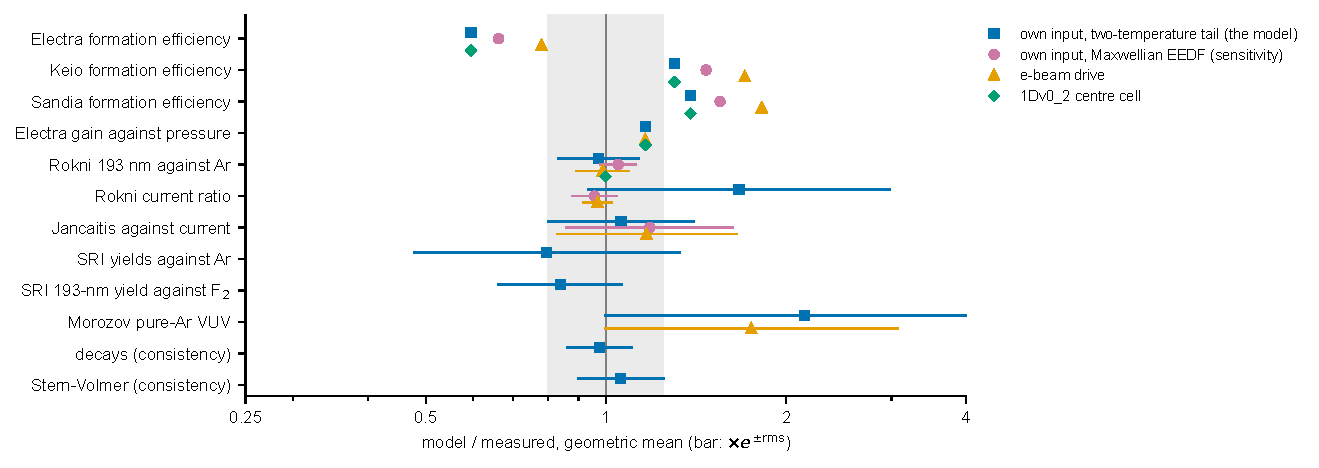
\includegraphics[width=\linewidth]{figures/fig_scorecard}
\caption{Every test at a glance, model over measured on a logarithmic axis.
A bar spans the geometric mean times $e^{\pm\mathrm{rms}}$ where a test has
three points or more. The grey band is 0.8 to 1.25.}
\label{fig:score}
\end{figure}

\section{How the numbers were made}

Each dataset has one role. The decays and Stern-Volmer plots that the
network's constants were read from check that the network reproduces them.
Every other measurement is held out and scores the model. No dataset sets a
rate, and no band is narrowed or moved by a score. This is the repository's
predictive-only policy. A score is the ratio of model to measurement. For a
set it is the geometric mean with the rms of the natural logarithms, and a
relative curve leaves out its normalisation point.

Each test runs v0\_2 three ways. LIGHT's own input puts the pump into the
electron gas, and the two-temperature closure reads a tail table made from
beam-sustained kinetic solutions. This is the model, and every score is its
score unless a column says otherwise. The same input on a Maxwellian EEDF
shows how much of a result the tail table makes. The electron-beam drive in
\path{v0_2/beam.py} deposits the same power as ion pairs, excited atoms and
secondary electrons. It runs REBUILD's Spencer-Fano cascade on the model's
own cross sections with the measured secondary spectrum of Opal, Peterson and
Beaty, $\bar E$ = \wi{beam.ebar}\unit{eV} for argon, and gives
\wi{beam.W}\unit{eV} per ion pair and \wi{beam.exc} excited atoms per pair
at the reference fill, with \wi{beam.eps}\unit{eV} per pair to the
electrons. W is an output, scored against the measured
\wi{beam.Wlit}\unit{eV} and \wi{beam.Wmiss}\,\% under it in pure argon.
REBUILD's own rule, equal sharing read at one source energy, gives
\wi{beam.rebW}\unit{eV} and \wi{beam.rebexc}, a point on an oscillation
that the measured spectrum removes. The seeded starts of SRI and Chen and
Payne take the drive's excited atoms per ion. 1Dv0\_2 runs both inputs on
\wi{od.cells} cells, the beam's products added in every cell of its stage.

Every number in this note is written by \path{make_overview.py} from the
records of \path{arf_data/score_arf.py}, made with the chemistry this
note describes, and from fresh runs. \path{v0_2/tests/test_docs.py}
fails when the generated files no longer match the network or the scores.

\section{The ArF network}

v0\_2 keeps KrF v0\_2's equations, energy ledger, two-temperature closure and
bands. Its species, cross sections, tail table and rates are ArF's. Five
things differ from KrF.
\begin{itemize}
\item One excimer state. No ArF C position, B--C mixing rate or equilibrium
  is measured, and the calculated B--C splitting is about 0.25\unit{eV}.
  \ArFs{} is ArF(B) alone.
\item Stern-Volmer products. The ArF(B) radiative lifetime has never been
  measured, and its \wi{rates.tauB}\unit{ns} is Dunning and Hay's
  calculation. The quenching of ArF(B) by \Ft{}, Ar, 2Ar and electrons is
  measured as products $k\tau_B$, and the rows divide them by $\tau_B$. A
  change of the calculated lifetime keeps every measured product.
\item The harpoon yield. \Ars{} + \Ft{} makes \ArFs{} with yield 0.5,
  Setser's flowing-afterglow measurement, where every published ArF model
  books 1.0.
\item The argon levels. Each of the \wi{rates.nAr} excitation blocks of the
  IST-Lisbon set is its own row. The \wi{rates.nAr4s} 4s blocks make \Ars{},
  and the \wi{rates.nArHi} higher ones cascade to it at once.
\item Ion-ion recombination. No absolute measurement exists. The rows use
  Hoffman and Moreno's calculation as Lee 1989 prints it, with the Debye
  screening and the Thomson $(T_g/300)^{-3}$ that KrF's rows carry.
\end{itemize}
The network carries \wi{rates.nBands} bands, \wi{rates.nZero} of them for
rates with no measurement. Appendix~A lists every row, band and species
energy.

\section{The reference point}

At the reference point, \wi{ref.p}\unit{atm} with \wi{ref.f2}\,\% \Ft{} and
\wi{ref.kw}\unit{kW/cm^3} for \wi{ref.pulse}\unit{\mu s} followed to
\wi{ref.tend}\unit{\mu s}, v0\_2 radiates \wi{ref.e193}\,\% of the deposited
energy at 193\unit{nm} (Table~\ref{tab:budget}). The ArF(B) formed carries
\wi{ref.formed}\,\% of the input as 193-nm quanta. It comes \wi{ref.chharp}\,\%
from \Ars{} + \Ft{}, \wi{ref.chdimer}\,\% from \Arts{} + \Ft{} and
\wi{ref.chion}\,\% from ion-ion recombination. Of the ArF(B) formed,
\wi{ref.arf.rad}\,\% radiates, \wi{ref.arf.tri}\,\% forms \AtF{},
\wi{ref.arf.qar}\,\% is quenched by Ar and \wi{ref.arf.qf}\,\% by \Ft{}. Of
the \Ars{} formed, \wi{ref.ars.harp}\,\% makes ArF(B), \wi{ref.ars.rest}\,\%
reacts with \Ft{} without making it and \wi{ref.ars.dimer}\,\% forms \Arts{}.
The \Ft{} falls below a tenth of its fill at \wi{ref.burn}\unit{ns}. $T_e$
averages \wi{ref.te}\unit{eV} over the pulse and $T_g$ ends at
\wi{ref.tg}\unit{K}. The ledger closes to \wi{ref.closure} of the input.

On a Maxwellian EEDF the same point gives \wi{ref.m193}\,\% at 193\unit{nm}
at a mean $T_e$ of \wi{ref.mte}\unit{eV}. The seed density sets only the
first nanoseconds, and seeds of \wi{ref.seedlo} to
\wi{ref.seedhi}\unit{cm^{-3}} give \wi{ref.seeds}\,\%.

\begin{table}[h]
\centering\footnotesize
\begin{tabular}{@{}lr@{}}
\toprule
where the deposited energy is at the end & \% of the input\\
\midrule
\wiTBudget
\bottomrule
\end{tabular}
\caption{The reference point's energy at \wi{ref.tend}\unit{\mu s}. The
stored entries are formation energy still held. The ledger closes to
\wi{ref.closure}.}
\label{tab:budget}
\end{table}

\section{The bands}

Each band at either end, the others at their defaults, gives
Table~\ref{tab:bands}. Three rates are the levers at the reference point.
\Arts{} + F, which has no measurement, takes the 193-nm share from
\wi{ref.e193} to \wi{band.ar2f.hi}\,\% at the top of its band. The \ArFs{}
yield of \Ars{} + \Ft{} spans \wi{band.arfyield.lo} to
\wi{band.arfyield.hi}\,\%. The trimer's $k\tau_B$ spans
\wi{band.arftrimer.hi} to \wi{band.arftrimer.lo}\,\%, and the trimer's gas
temperature law at the bottom of its band gives \wi{band.trimertgpow.lo}\,\%.
\Ars{} + 2Ar spans \wi{band.ar2form.lo} to \wi{band.ar2form.hi}\,\%, and every
other band moves the 193-nm share by \wi{band.othermax} percentage points or
less.

\begin{table}[h]
\centering\footnotesize
\begin{tabular}{@{}lrrrrrr@{}}
\toprule
band & low end & 193\unit{nm}, \% & 127\unit{nm}, \% & high end &
  193\unit{nm}, \% & 127\unit{nm}, \%\\
\midrule
\wiTBandEnds
\bottomrule
\end{tabular}
\caption{The reference point with one band at a time at either end of its
range. At the defaults 193\unit{nm} takes \wi{ref.e193}\,\% and 127\unit{nm}
\wi{ref.e127}\,\%. Appendix~A.3 gives each band's source and units.}
\label{tab:bands}
\end{table}

\section{Formation efficiency and gain at the lasers}

A published small-signal gain $g_0$ and saturation intensity
$I_\mathrm{sat}$ give a formation efficiency that needs no cross section,
\gIP{}. It is the ArF(B) formation rate times the 193-nm quantum over the
deposited power at the quasi-steady peak, and v0\_2 makes the same quantity
from its formation rate in the pulse's window (Figure~\ref{fig:form}).

At Electra's \wi{elf.x1p}\unit{MW/cm^3}, the measured \wi{elf.meas1} is met at
\x{\wi{elf.r1}} on the own input and \x{\wi{elf.br1}} under the beam drive.
With the \ArFs{} yield at 1.0 the own input gives \x{\wi{ely.r}} and the beam
drive \x{\wi{ely.br}}, so the measured yield of 0.5 and the published
models' 1.0 bracket Electra. Keio's printed pump gives \x{\wi{keio.r1}} and
Sandia's abstract \x{\wi{san.r1}}. NRL replots Keio's point at
\wi{keio.x2p}\unit{MW/cm^3}, which would make it \x{\wi{keio.r2}}, so Keio's
pump reading decides whether v0\_2 is low or high there.

Electra's single-pass gain falls to \wi{elt.meas} of its
\wi{elt.loatm}-atm value at \wi{elt.hiatm}\unit{atm}, and v0\_2's falls to
\wi{elt.mod} (Table~\ref{tab:electra}). Wolford notes that Electra's beam is
not uniform at low pressure. The gain itself needs the ArF(B) stimulated
emission cross section, which is only calculated. With Lee's value v0\_2's
$g_0$ is in the last column.

\begin{figure}[h]
\centering
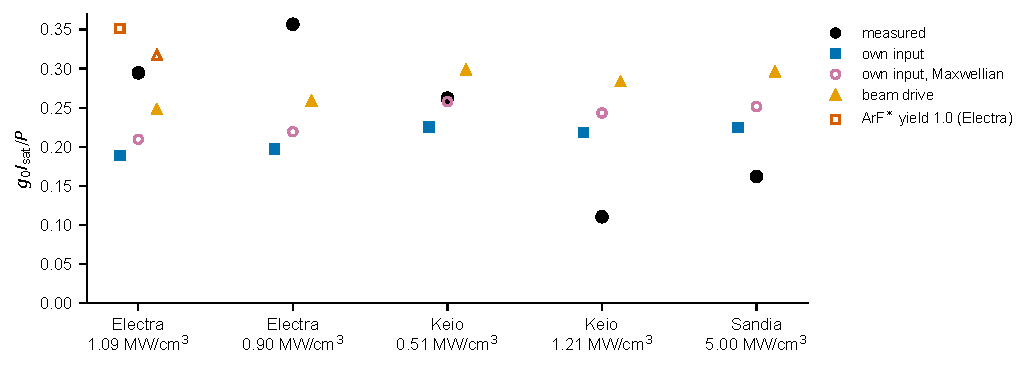
\includegraphics[width=0.94\linewidth]{figures/fig_formation}
\caption{Formation efficiency \gIP{} at the three lasers. Open symbols are
the own input on a Maxwellian EEDF and, at Electra's
\wi{elf.x1p}\unit{MW/cm^3}, the \ArFs{} yield at 1.0.}
\label{fig:form}
\end{figure}

\begin{table}[h]
\centering\footnotesize
\begin{tabular}{@{}rrrrrrr@{}}
\toprule
atm & $g_0$ measured, \%/cm & measured & own input & beam drive & 1Dv0\_2
  centre & $g_0$ with Lee's $\sigma$, \%/cm\\
\midrule
\wiTElectraTrend
\bottomrule
\end{tabular}
\caption{Electra's single-pass gain against pressure, each column relative
to its value at \wi{elt.loatm}\unit{atm}. The model's ratios are its ArF(B)
density ratios and need no cross section.}
\label{tab:electra}
\end{table}

\section{Fluorescence against pressure and current}

Rokni, Jacob and Mangano measured the steady 193-nm fluorescence under a
5-A/cm$^2$ beam with 2\unit{Torr} of \Ft{} from \wi{rkp.xmin} to
\wi{rkp.xmax}\unit{atm} of argon (Figure~\ref{fig:rokni}). Normalised at
1\unit{atm}, v0\_2 follows it with an rms of \wi{rkp.ownrms} in the logarithm
on its own input and \wi{rkp.beamrms} under the beam drive. The deposition
is taken as \wi{rkp.pw}\unit{kW/cm^3} per atm, an estimate, which sets the
regime of the own input and not the normalised curve. In the same paper a
current changed \x{25} changes the fluorescence by \wi{rkc.meas}, the ion
channel forming \ArFs{} with branching near one. The beam drive gives
\wi{rkc.beam} of that, and the own input \wi{rkc.own}
(Table~\ref{tab:rkc}). Section~\ref{sec:closure} gives the reason.

\begin{figure}[h]
\centering
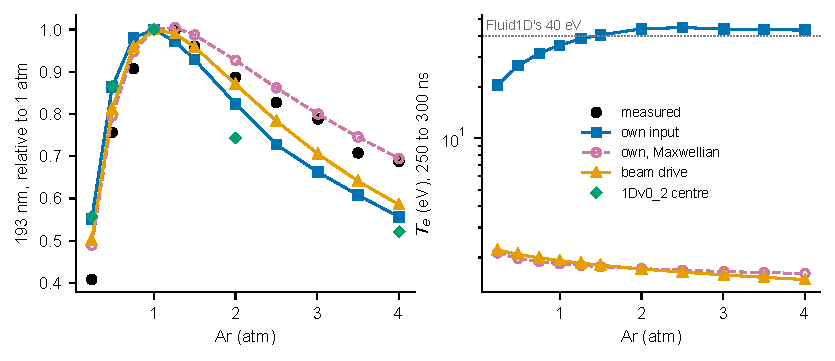
\includegraphics[width=\linewidth]{figures/fig_rokni}
\caption{Rokni 1977 Fig.~4. Left, the 193-nm fluorescence against argon
pressure, relative to 1\unit{atm}. Right, the model's $T_e$ over the last
50\unit{ns} of the 300-ns pulse.}
\label{fig:rokni}
\end{figure}

\begin{table}[h]
\centering\footnotesize
\begin{tabular}{@{}rrrrrrrrr@{}}
\toprule
& & \multicolumn{3}{c}{own input} & \multicolumn{2}{c}{own, Maxwellian} &
  \multicolumn{2}{c}{beam drive}\\
\cmidrule(lr){3-5}\cmidrule(lr){6-7}\cmidrule(l){8-9}
Ar, atm & measured & ratio & $T_e$, eV & $T_e$ at 1/25 & ratio & $T_e$, eV &
  ratio & $T_e$, eV\\
\midrule
\wiTRokniRatio
\bottomrule
\end{tabular}
\caption{Rokni 1977 Fig.~5, the 193-nm fluorescence ratio for a \x{25}
change of the beam current, with the model's mean $T_e$ over 250 to
300\unit{ns} at the full current, and at 1/25 of it for the own input.}
\label{tab:rkc}
\end{table}

Jancaitis and Powell measured the peak \ArFs{} and \AtF{} fluorescence
against the beam's current density from \wi{jan.jmin} to
\wi{jan.jmax}\unit{A/cm^2} (Figure~\ref{fig:jan}). v0\_2's \ArFs{} peak
follows the measured one with an rms of \wi{jan.frms} in the logarithm, and
at
\wi{jan.fxtop}\unit{A/cm^2} it is \x{\wi{jan.ftop}}. Its \AtF{} keeps rising
where the measured one saturates, \x{\wi{jan.aone}} and \x{\wi{jan.atwo}} at
\wi{jan.axone} and \wi{jan.axtwo}\unit{A/cm^2}. Jancaitis attributes the
saturation to a loss of \AtF{} that grows with the excitation. He estimates
it as \AtF{} + \el{}, which is not measured, and the network does not carry
it.

\begin{figure}[h]
\centering
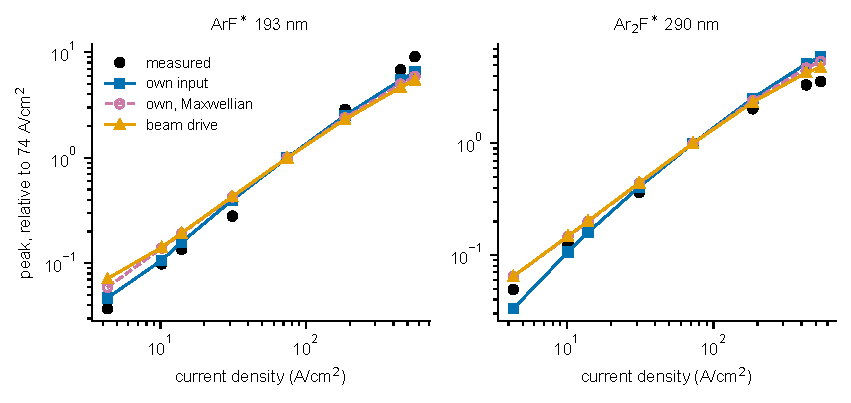
\includegraphics[width=\linewidth]{figures/fig_jancaitis}
\caption{Jancaitis 1983 Fig.~3, peak fluorescence against current density,
each curve relative to its point nearest 74\unit{A/cm^2}.}
\label{fig:jan}
\end{figure}

\section{Photons per initial excitation}

SRI measured the photons at 193 and 290\unit{nm} per ion and excited atom
made by a 3-ns Febetron pulse, against argon and against \Ft{}
(Figure~\ref{fig:sri}). v0\_2 starts from SRI's excitation and follows the
afterglow. Its 193-nm yield is \wi{sria.agm} of the measured against argon,
\wi{sria.arng} over the \wi{sria.an} points, and \wi{srif.own} against \Ft{},
\wi{srif.rng}. The model makes too little \ArFs{} per excitation, the same
question as at Electra. Its 290-nm \AtF{} yield runs from \x{\wi{sria.blo}} at
\wi{sria.bloatm}\unit{atm} to \x{\wi{sria.bhi}} at \wi{sria.bhiatm}\unit{atm},
too little \AtF{} at low pressure and too much at high pressure. At high
pressure, as at Jancaitis's high currents, the network lacks a loss of
\AtF{}.

\begin{figure}[h]
\centering
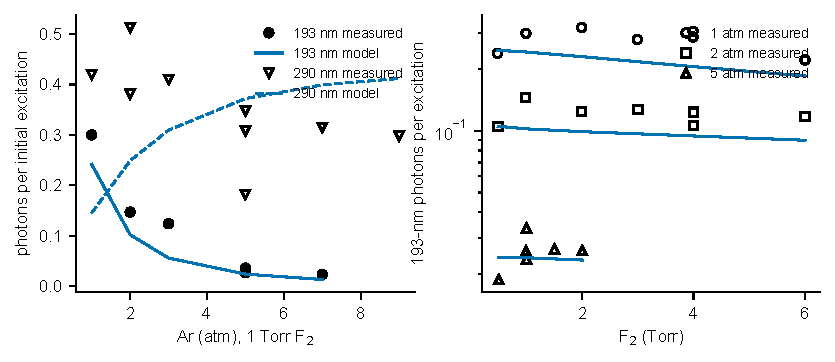
\includegraphics[width=\linewidth]{figures/fig_sri}
\caption{SRI MP-76-99. Left, Fig.~4, the yields against argon at
1\unit{Torr} of \Ft{}. Right, Fig.~11, the 193-nm yield against \Ft{} at 1,
2 and 5\unit{atm}. Lines are v0\_2.}
\label{fig:sri}
\end{figure}

\section{Pure argon}

Morozov and coworkers measured the VUV power of pure argon under a
low-energy beam at \wi{moz.meas} $\pm$ \wi{moz.err} of the deposited power,
independent of pressure from 500 to 1400\unit{hPa} (Figure~\ref{fig:moz}).
Under the beam drive v0\_2 turns each ion and excitation into one \Arts{}
photon, \wi{moz.bplat} of the input, and its own input gives \wi{moz.oplat}.
The measurement is \wi{moz.frac} of the beam drive's value, and no band
closes the gap. At 1000\unit{hPa} the ends of the \Ars{} and \Arts{} bands
give \wi{mozb.min} to \wi{mozb.max} under the beam drive, the lowest with
\wi{mozb.minband} at its top. KrF's pure-krypton check misses the same way.
The missing loss is not in the network. The drive's \wi{beam.W0}\unit{eV}
per pair in pure argon puts the ceiling at \wi{beam.ceil}, near the 0.53
Morozov quotes as the theoretical maximum. He finds his krypton and xenon
close to their maxima and his argon at 62\,\% of it, so no input closes the
gap. Either the network lacks an argon VUV loss that has been measured, or
his argon value is low.

\begin{figure}[h]
\centering
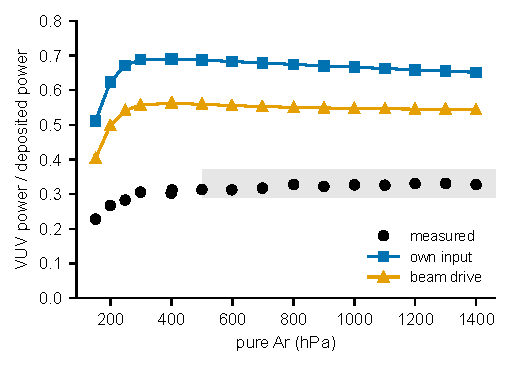
\includegraphics[width=0.56\linewidth]{figures/fig_morozov}
\caption{Morozov 2008 Fig.~10, pure-argon VUV power over deposited power.
The grey band is the printed \wi{moz.meas} $\pm$ \wi{moz.err}.}
\label{fig:moz}
\end{figure}

\section{The sources of the constants}

The network's constants are means of the groups that measured them. Run
back against those measurements, v0\_2 reproduces the decays with a
geometric mean of \wi{dec.own} and an rms of \wi{dec.ownrms} over
\wi{dec.n} points, and the Stern-Volmer plots with \wi{sv.own} and
\wi{sv.ownrms} (Table~\ref{tab:cons}). Rokni's \Ft{} plot, \x{\wi{sv.rokni}},
is a steady e-beam run on the own input at a low pump, where
Section~\ref{sec:closure} applies. These are checks of the bookkeeping, not
of accuracy.

\begin{table}[h]
\centering\footnotesize
\begin{tabular}{@{}lrrr@{}}
\toprule
set & points & model over measured & rms of the logarithm\\
\midrule
\wiTDecays
\midrule
\wiTSV
\bottomrule
\end{tabular}
\caption{The decays and Stern-Volmer plots the constants came from.}
\label{tab:cons}
\end{table}

\section{The electron closure and the input}
\label{sec:closure}

LIGHT's own input puts the pump into the electrons' bulk. The
two-temperature closure gives the argon rows a tail above
\wi{rates.ebreak}\unit{eV} at $T_\mathrm{tail} = r\,T_e$, with $r$ read from
a table made from beam-sustained kinetic solutions. The table was checked
against those solutions where $n_e/N$ is at least $10^{-6}$. Rokni's runs sit
near $n_e/N$ = \wi{tr.nen}, where the table gives $r$ = \wi{tr.tail}. With so
cold a tail the bulk has to reach \wi{rkp.te}\unit{eV} before the tail
excites enough to take the pump. On a Maxwellian EEDF the same runs sit at
\wi{rkpM.te}\unit{eV}, where the beam drive sits at \wi{rkp.bte}\unit{eV}
(Table~\ref{tab:te}). The Maxwellian own input also follows Rokni's pressure
curve more closely, \x{\wi{rkpM.rlo}}, \x{\wi{rkpM.rtwo}} and
\x{\wi{rkpM.rfour}} at \wi{rkp.plo}, \wi{rkp.ptwo} and
\wi{rkp.pfour}\unit{atm} against \x{\wi{rkp.rlo}}, \x{\wi{rkp.rtwo}} and
\x{\wi{rkp.rfour}} with the tail, and it gives the ratio for \x{25} in
current at \x{\wi{rkcM.own}} against \x{\wi{rkc.own}}, as the beam drive's
\x{\wi{rkc.beam}} does. At the gain points the pump is higher, the
tail warmer and the difference smaller. Electra goes from \x{\wi{elf.r1}} to
\x{\wi{elfM.r1}}.

The own input's scores at low pumps are therefore the tail table's as much
as the network's. The beam drive, whose secondaries carry the excitation,
does not depend on it.

\begin{table}[h]
\centering\footnotesize
\begin{tabular}{@{}lrrr@{}}
\toprule
runs & own input & own input, Maxwellian & beam drive\\
\midrule
\wiTTeRegimes
\bottomrule
\end{tabular}
\caption{The model's $T_e$ in eV, over 250 to 300\unit{ns} at Rokni's
conditions, 20 to 50\unit{ns} at Jancaitis's and in the formation window at
the gain points.}
\label{tab:te}
\end{table}

\section{The 1-D model}

1Dv0\_2 runs v0\_2's chemistry, byte for byte, in each cell of Fluid1D's gap.
At the device points its centre cell gives v0\_2's numbers to \wi{od.dev},
the largest at \wi{od.devtest}, and its gap average lies \wi{od.gap}\,\%
lower on \wi{od.cells} cells. The difference is the wall cells, whose sheaths
the mesh does not resolve. Table~\ref{tab:mesh} gives the reference point on
\wi{ma.cells} and \wi{mb.cells} cells. The centre cell agrees with v0\_2 to
\wi{ma.centredev} and \wi{mb.centredev}. In the wall cells the mean-energy
bounds cut \wi{ma.cut} and \wi{mb.cut}\,\% of the input, Fluid1D's split keeps
out phantom negative field work of \wi{ma.phantom} and \wi{mb.phantom}\,\%,
and \wi{ma.walls} and \wi{mb.walls}\,\% is lost to the walls. Under the
beam the 1-D stage adds the beam's ion pairs, with their electrons, excited
atoms and prompt \Ft{} dissociations, in every cell and substep, and its
centre cell gives v0\_2's beam numbers to \wi{od.bdev}, the largest at
\wi{od.bdevtest}, with the gap average \wi{od.bgap}\,\% lower. The own
input's 1-D runs are unchanged by it, bit for bit.

\begin{table}[h]
\centering\footnotesize
\begin{tabular}{@{}lrrrrr@{}}
\toprule
& v0\_2 & \multicolumn{2}{c}{\wi{ma.cells} cells} &
  \multicolumn{2}{c}{\wi{mb.cells} cells}\\
\cmidrule(lr){3-4}\cmidrule(l){5-6}
& & centre & gap & centre & gap\\
\midrule
\wiTMesh
\bottomrule
\end{tabular}
\caption{The reference point in v0\_2 and in 1Dv0\_2 on two meshes.}
\label{tab:mesh}
\end{table}

Fluid1D holds the mean electron energy at or below \wi{tr.eps}\unit{eV}, a
$T_e$ of \wi{tr.ceil}\unit{eV}. Where v0\_2's $T_e$ passes it, at Rokni's
\wi{rkp.ptwo} and \wi{rkp.pfour}\unit{atm} with \wi{rkp.te2} and
\wi{rkp.te4}\unit{eV}, 1Dv0\_2's centre gives \x{\wi{rkp.dep2}} and
\x{\wi{rkp.dep4}} of v0\_2. Under the beam v0\_2's $T_e$ stays at
\wi{rkp.bte}\unit{eV} over all of Rokni's pressures, and at these two the
centre gives \x{\wi{rkp.bdep2}} and \x{\wi{rkp.bdep4}} of v0\_2's beam run.
Figure~\ref{fig:trace} follows the
own input's \wi{rkp.ptwo}-atm run. From \wi{tr.from}\unit{ns} the centre cell and
v0\_2 agree to \wi{tr.agree}\,\% in every species but \Arp{} until their
electron temperatures part by \wi{tr.partpct}\,\% at \wi{tr.tpart}\unit{ns},
as the 1-D $T_e$ reaches the ceiling. \Arp{}, whose production is steep in
$T_e$, already differs by \wi{tr.arpagree}\,\% at that moment. After it
v0\_2's $T_e$ climbs to \wi{tr.te0}\unit{eV}. Above the \wi{rates.temax}-eV edge of the rate
tables the rows on Maxwellian tables are held, but the tail rows follow
$T_\mathrm{tail} = r\,T_e$, which stays far below the edge. At this state
$r$ = \wi{tr.tail}, and the ionization rate C2 is \wi{tr.ctwo.thirty} at
\wi{rates.temax}\unit{eV}, \wi{tr.ctwo.forty} at \wi{tr.ceil}\unit{eV} and
\wi{tr.ctwo.end}\unit{cm^3s^{-1}} at v0\_2's \wi{tr.te0}\unit{eV}. v0\_2's
ionization keeps rising while the 1-D's is held, and by 300\unit{ns} v0\_2
holds \wi{tr.arp} times the 1-D's \Arp{}. Holding the \Artp{} + \el{} power
law at its \wi{rates.temax}-eV value in v0\_2, as the 1-D stage does, moves
the emission by \wi{rclip.dev}\,\% or less.

\begin{figure}[h]
\centering
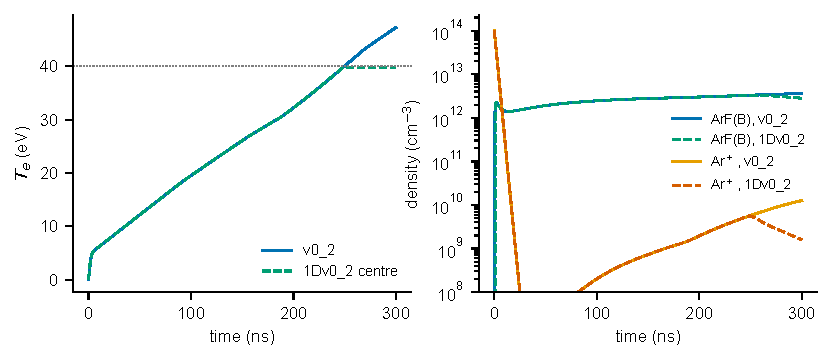
\includegraphics[width=\linewidth]{figures/fig_trace}
\caption{Rokni's \wi{rkp.ptwo}-atm run in v0\_2 and in 1Dv0\_2's centre cell.
Left, $T_e$ and Fluid1D's ceiling. Right, ArF(B) and \Arp{}.}
\label{fig:trace}
\end{figure}

\section{The energy ladder}

Figure~\ref{fig:ladder} places every species of v0\_2 at its formation
energy, the energy above ground-state Ar and \Ft{} at rest that
Appendix~A lists, and draws the rows that move energy between them. It is
LIGHT's ladder with v0\_2's own numbers. ArF(B) lies \lad{DeB}\unit{eV}
below the ion pair \Arp{} + \Fm{} and \lad{BoverArF}\unit{eV} above Ar + F,
exactly the \lad{wl.G4}-nm quantum of \lad{hv.G4}\unit{eV}, so the photon
leaves ArF(X) with \lad{heat.G4}\unit{eV} to heat. The harpoon G3 heats the
gas by \lad{heat.G3}\unit{eV} for each ArF(B) it makes, \Arts{} + \Ft{}
through NK7 by \lad{heat.NK7}\unit{eV}, the ion-ion recombinations K26 and
K108 by \lad{heat.K26} and \lad{heat.K108}\unit{eV}, and the trimer's
formation by \lad{heat.G5}\unit{eV}. \AtF{} emits \lad{hv.C3}\unit{eV} at
\lad{wl.C3}\unit{nm} and leaves \lad{heat.C3}\unit{eV} of lower-state
repulsion, and \Arts{} emits \lad{hv.V}\unit{eV} at \lad{wl.V}\unit{nm} and
leaves \lad{heat.V}\unit{eV}. The \lad{nG1} G1 rows excite the 4s levels,
with thresholds from \lad{g1.lo} to \lad{g1.hi}\unit{eV}, and the
\lad{nC1} C1 rows the higher levels, from \lad{c1.lo} to
\lad{c1.hi}\unit{eV}. Each family is drawn as one arrow.

\begin{figure}[p]
\centering
\ladpicture
\caption{The energy ladder of LIGHT\_ArF\_ebeam v0\_2, version \lad{version}, in
eV above ground-state Ar and \Ft{} at rest. A bar is a species at its
formation energy and a dashed bar a pair, the sum of two. An arrow is a
row, labelled with its id. It is solid in the default network and dotted
for a band whose default is 0, \lad{zero}. The rows of the optional group
\lad{groups} are dashed. A photon's arrow drops by its quantum, and the red
squiggle below it is the heat its lower state gives the gas as it falls
apart. A red stub is a quench. The energy a row releases heats the gas,
except a photon's, which leaves, and that of \lad{toe}, which goes to the
electrons. The \lad{nG1} 4s rows and the \lad{nC1} higher rows are each
drawn as one arrow to their highest threshold, and the squiggle beside
each is the heat of the levels above \Ars. The rows \lad{notdrawn} move
nothing between levels and are not drawn.}
\label{fig:ladder}
\end{figure}

\section{The system map}

The map on page~\pageref{p:map} draws v0\_2's basic network at the reference
point, \wm{p}\unit{atm} of Ar with \wm{xF2}\,\% F$_2$,
\wm{P}\unit{kW\,cm^{-3}} for \wm{pulse}\unit{\mu s}, with $n_e$ seeded at
$\wm{ne}$\unit{cm^{-3}} and then free and every band at its default. Band
widths are proportional to the energy they carry, and energy is conserved
at each of the map's \wm{nodes} nodes to within $10^{-8}$ of \Edep. Of the
deposited energy, \wm{arf.eff}\,\% passes through ArF(B) in
\wm{hv.G4}-eV quanta. Of that ArF(B), \wm{brf.G4}\,\% radiates at
193\unit{nm}, \wm{brf.tri}\,\% forms the trimer and \wm{brf.Ar}\,\% is
quenched by argon, so
\wm{out.193}\,\% of the deposited energy leaves at 193\unit{nm}, and
\wm{out.127}\,\% leaves at 127\unit{nm} from \Arts. A further
\wm{out.other}\,\% is still held at \wm{tend}\unit{\mu s}, most of it in
\Arts, whose radiative lifetime is \wm{tauRAD}\unit{\mu s}.

\section{Where LIGHT\_ArF\_ebeam is not yet reliable}

\begin{enumerate}[leftmargin=1.6em]
\item The \ArFs{} made per excitation. Electra at \x{\wi{elf.r1}} on the
  own input and \x{\wi{elf.br1}} under the beam, SRI's
  193-nm yield at \wi{sria.agm} and the yield band that brackets Electra all
  point to it. The measured yield 0.5 stays the default. A measurement of the
  \ArFs{} yield of \Ars{} + \Ft{} near 1\unit{atm} would settle it.
\item The loss of \AtF{}. The network has no \AtF{} + \el{} and no other loss
  that grows with excitation. Jancaitis's \AtF{} and SRI's 290-nm yield at
  high pressure call for one.
\item Pure argon. The VUV efficiency is \wi{moz.frac} of the one-photon
  value, and no band closes it.
\item The electron closure at low pumps. The tail table is read below the
  ionization fractions it was checked at, and the own input's results there
  depend on it (Section~\ref{sec:closure}). The beam drive does not.
\item The formation efficiency against pump. Under the beam the model makes
  \ArFs{} at nearly the same share of the input at every device pump, where
  the measured share falls from Electra to Sandia, and Sandia rises to
  \x{\wi{san.br1}}.
\item Electra's gain against pressure, measured to fall faster than v0\_2's.
\item What was never measured. The ArF(B) radiative lifetime, the ArF C
  state, \Arts{} + F and the Penning rates are calculations or bands. F + F +
  Ar is known here only through Baulch 1981. Sandia's efficiency is from its
  abstract, and Keio's two pump readings give \x{\wi{keio.r1}} and
  \x{\wi{keio.r2}}.
\end{enumerate}

% The map page closes the main text, so the text runs on past the
% ladder's float page and no page is left short. \includepdf breaks the
% page, and an \afterpage map would fire inside Appendix A's longtables and
% hang pdfTeX (Known-bad).
\clearpage
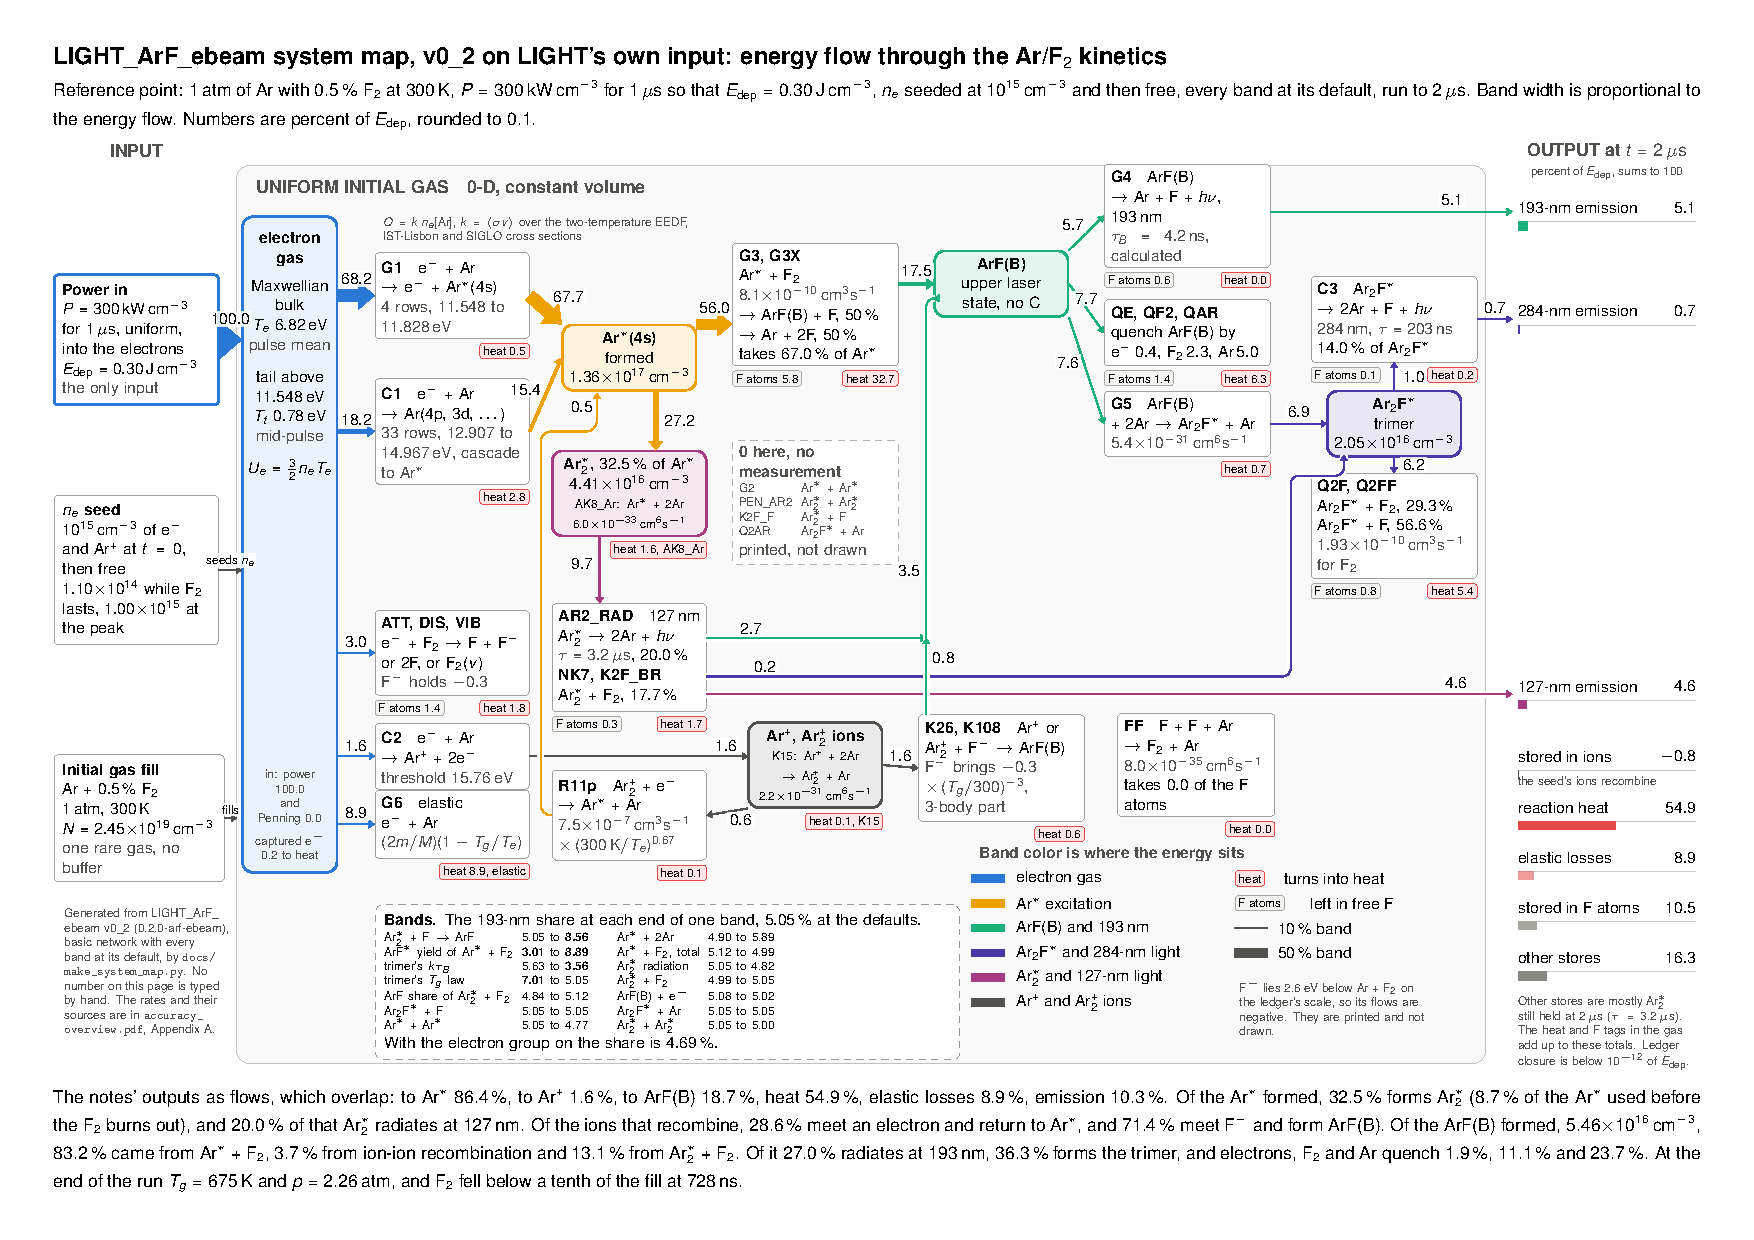
\includepdf[pages=1,fitpaper=true,
  pagecommand={\thispagestyle{empty}\label{p:map}}]{system_map.pdf}

\appendix
\section{The reaction rates}

\subsection{The basic network, \wi{rates.nBasic} rows}
Rates at 300\unit{K}. A band row runs its band's default. $N$ is the gas
density in amagat.
{\footnotesize
\begin{longtable}{@{}>{\raggedright\arraybackslash}p{1.8cm}
  >{\raggedright\arraybackslash}p{3.7cm}>{\raggedright\arraybackslash}p{3.9cm}
  >{\raggedright\arraybackslash}p{1.9cm}>{\raggedright\arraybackslash}p{3.3cm}@{}}
\toprule
row & reaction & rate & depends on & source\\
\midrule
\endhead
\wiTRows
\bottomrule
\end{longtable}}

\subsection{The optional electron group, \wi{rates.nGroup} rows, off by
default}
{\footnotesize
\begin{longtable}{@{}>{\raggedright\arraybackslash}p{1.8cm}
  >{\raggedright\arraybackslash}p{3.7cm}>{\raggedright\arraybackslash}p{3.9cm}
  >{\raggedright\arraybackslash}p{1.9cm}>{\raggedright\arraybackslash}p{3.3cm}@{}}
\toprule
row & reaction & rate & depends on & source\\
\midrule
\wiTGroup
\bottomrule
\end{longtable}}

\subsection{The bands}
{\footnotesize
\begin{longtable}{@{}>{\raggedright\arraybackslash}p{2.1cm}
  >{\raggedright\arraybackslash}p{3.3cm}>{\raggedright\arraybackslash}p{1.6cm}
  >{\raggedright\arraybackslash}p{2.9cm}>{\raggedright\arraybackslash}p{1.1cm}
  >{\raggedright\arraybackslash}p{3.0cm}@{}}
\toprule
band & rate & default & range & unit & source\\
\midrule
\endhead
\wiTBandList
\bottomrule
\end{longtable}}

\subsection{Formation energies}
{\footnotesize
\begin{longtable}{@{}lrll@{}}
\toprule
species & eV above Ar + \Ft{} & how known & source\\
\midrule
\wiTSpecies
\bottomrule
\end{longtable}}

\section{The data scored}

The \wi{readings.n} figure readings in \path{arf_data/fig_readings/}, each
with its source and the way it was read. The numbers printed in the sources'
text are in \path{arf_data/SCORING_DATA.md}.
{\footnotesize
\begin{longtable}{@{}>{\raggedright\arraybackslash}p{3.2cm}
  >{\raggedright\arraybackslash}p{8.3cm}>{\raggedright\arraybackslash}p{3.6cm}@{}}
\toprule
file & source & reading\\
\midrule
\endhead
\wiTReadings
\bottomrule
\end{longtable}}

\end{document}
